\chapter{Statistical Analysis and Parameter Selection}
\label{chap:MapperStatistic}



In Chapters~\ref{chap:backgroundTelescopesReeb} and~\ref{chap:MapperStability}, we have seen
how Reeb graphs and Mappers can be compared with adequate metrics, when they are computed on 
non discrete topological spaces. In this chapter, we focus on Mappers 
computed on discrete and finite topological spaces, i.e. point clouds.
In particular, we provide approximation results (Theorems~\ref{th:sig-approx} and~\ref{th:sig-approx-general}) 
controlling the distance between Mappers computed on discrete and non discrete topological spaces.
Moreover, we show that {\em interval-} and {\em intersection-crossing edges} are the principal
responsibles of discretization artifacts (Lemma~\ref{lem:cons_equ} and~\ref{lem:cons_equ2}).
This observation allows us to study the rate of convergence of the Mapper to 
the Reeb graph when the cardinality of the point cloud grows to $+\infty$.

Our main result is Proposition~\ref{prop:UpBdRestr}, which states that
 the rate of convergence of the Mapper, when computed on a point cloud $X_n$ drawn from a specific probability distribution whose support is a compact Riemannian manifold embedded in $\R^D$, 
is of the order $({\rm log}(n)/n)^{1/d}$:
$$ \mathbb{E}\left[\distb(\Mapper_f(X_n,\I_n),\Reeb_f(X))\right]\lesssim C\omega\left(\left(\frac{{\rm log}(n)}{n}\right)^{\frac 1d}\right),$$
where $n$ is the cardinality of the point cloud, $C$ is a constant, $\omega$ is a measure of the regularity of $f$ (for instance $\omega(x)=cx$
when $f$ is Lipschitz with constant $c$),
and $\I_n$ is a specific cover that depends only on $X_n$. 
We show that this rate is minimax optimal, meaning that no other estimator of the Reeb graph
can converge faster.

We finally use the specific cover $\I_n$ as a heuristic to automatically tune Mapper parameters,
and we build on the convergence result to compute confidence regions for the topological features of the Mapper,
hence providing statistical guarantees for all applications of Topological Data Analysis relying on Mapper,
such as clustering~\cite{Lum13,Nicolau11} and feature selection~\cite{Nielson15, Rucco15}.
   

%However, 
%
%

%

%

%Our main goal in this Chapter is to provide a statistical method to tune the parameters of Mapper automatically. 
%To select parameters for Mapper, or more generally to evaluate the significance of topological features provided by Mapper, 
%we develop a rigorous statistical framework for the convergence of the Mapper. This   
%is made possible by Section~\ref{sec:connection} of Chapter~\ref{chap:MapperStability} (in a deterministic setting),
%where we detailed a way to go from the input space to the Mapper using small perturbations. We build on this 
%relation between the input space and its Mapper to show that the Mapper is itself a measurable construction.
%In Section~\ref{sec:topoMultiNerve} of Chapter~\ref{chap:MapperStability}, we also showed that the topological structure 
%of the Mapper can actually be predicted from 
%the cover $\I$ by looking at appropriate extended persistence diagrams. In this Chapter, we use this observation, together with an approximation inequality, 
%to show that the Mapper, computed with a specific set of parameters, is actually
%an optimal estimator of its corresponding Reeb graph. Moreover, these specific parameters act as natural candidates 
%to obtain a reliable Mapper with no artifacts,
%avoiding the computational cost of testing millions of candidates and selecting the most stable ones in the brute-force setting of many practitioners.
%Finally, we also provide methods to assess the stability and compute confidence regions for the topological features of the Mapper.
%We believe that this set of methods open the way to an accessible and intuitive 
%utilization of Mapper for non expert researchers in applied topology.

\paragraph*{Plan of the Chapter.} In Section~\ref{sec:discrete}, we recall
how Reeb graphs and Mappers are computed on point clouds. Then,  %presents the necessary background 
%on the Reeb graph and Mapper, and it also 
we give an approximation inequality (Theorem~\ref{thm:geomineq}) for the Reeb graph in Section~\ref{sec:ApproxReeb}. 
From this approximation result, we derive rates of 
convergences as well as candidate parameters in Section~\ref{sec:ConfConv}, 
and we show how to get confidence regions in Section~\ref{sec:confR}. 
Section~\ref{sec:appli} illustrates the validity of our parameter tuning and
confidence regions with numerical experiments on smooth and noisy data.

%\paragraph*{Publications.} Section~\ref{sec:discrete} is taken from~\cite{Carriere15c}.
%The other Sections correspond to the article~\cite{Carriere17c}.

%\paragraph*{Convention.} In this chapter, we assume that 
%$X$ is a smooth and compact submanifold of $\R^d$, and
%we compute the Mapper on finite samples $P\subseteq X$
%using the 1-skeleton of the Rips complex built on top of $P$
%with parameter $\delta>0$, denoted by $\Rips_\delta^1(P)$, as in Section~\ref{sec:Mapper_constr}.
%Moreover, we assume that the gomic $\mathcal I$ is defined
%with intervals of constant length $r>0$
%and pairwise intersection length $gr$, $g\in\left[0,\frac12\left)$.
%To make this clear and avoid heavy notations, we use the shorthand $\Mapper_f(P,(r,g,\delta))$
%for $\Mapper_f(\Rips_\delta^1(P),\mathcal I)$.
%The length $r$ is called the {\em resolution} and the intersection length
%percentage $g$ is called the {\em gain}.


%%%%%%%%%%%%%%%%%%
\section{Approximations of (MultiNerve) Mappers and Reeb graphs}
\label{sec:discrete}

In this section, we discuss the approximation of the Reeb graph, the (MultiNerve) Mapper
and their signatures %~(\ref{eq:sign1}) 
when the pair $(X,f)$ is known
only through a finite set of sample points equipped with function
values. %We start with basic definitions in Section~\ref{sec:tools}, and give an approximation result for Reeb graphs in Section~\ref{sec:Reebapprox}.
%We then detail two discrete approximations for (MultiNerve) Mappers in Section~\ref{sec:Mapper_constr}.
%Their relationship is explained in Section~\ref{sec:approx-mapper}.
%Finally, we explicit all relationships between the different constructions in Section~\ref{sec:approx-sigs}.

\paragraph*{Convention.} From now on, we assume that the underlying space $\Xset$ 
is a compact Riemannian manifold of $\R^D$, %with intrinsic metric $d_X$,
$f:X\rightarrow\R$ is a Morse-type function and $\Xs_n=\{x_1,\cdots,x_n\}\subset X$ 
is a point cloud in~$X$ of cardinality $n\in\N$. Moreover, we let $\|\cdot\|$ denote the usual
Euclidean norm in $\R^D$. We often call $f$ a {\em filter} function, as in the literature 
on applications of Reeb graph and Mappers.

\subsection{Approximation tools}
\label{sec:tools}


\paragraph*{Rips complex.} All constructions take a neighborhood graph as
input, such as for instance the 1-skeleton graph of the Rips complex, defined as follows:
%
\begin{defin}
%Given $\delta\geq 0$ and a metric space $(X,d)$, 
Let $\delta \geq 0$ be a scale parameter.
The \emph{Rips complex} of $\Xs_n$ of parameter~$\delta$ is
the simplicial complex $\Rips_\delta(\Xs_n)$ defined by:
%
\[ 
\{x_{i_0},...,x_{i_k}\}\in\Rips_\delta(\Xs_n)\Leftrightarrow \|x_{i_p}-x_{i_q}\|\leq\delta\text{ for any }0\leq p,q\leq k,. 
\]
%
Its 1-skeleton graph is called the {\em Rips graph} of parameter~$\delta$ and denoted by~$\Rips_\delta^1(\Xs_n)$.

Moreover, given a geometric realization $|\Rips_\delta(\Xs_n)|$,
we let $\frips{f}:|\Rips_\delta(X_n)|\rightarrow\R$ denote the piecewise-linear
interpolation of $f$ along the simplices of $\Rips_\delta(X_n)$, and
%Since $|\Rips_\delta(\Xs_n)|$ is a metric space, 
we let $\Reeb_{\frips{f}}(|\Rips_\delta(X_n)|)$ 
denote its Reeb graph, with induced function $\frips{\freeb{f}}$.
\end{defin} 


\paragraph*{Geometric quantities.} Two geometric quantities that assess the smoothness of topological spaces
will be used in the hypotheses of the results in this chapter---see Theorem~\ref{th:Reebapprox} and Theorem~\ref{thm:geomineq}.
\begin{itemize}

\item {\em Reach.} The {\em medial axis} of $X\subset \R^D$ is the set of points in $\R^D$ with at least two nearest neighbors in $X$:
$${\rm med}(X)=\{y\in\R^D\,:\,{\rm card}\{x\in X\,:\,\|y-x\|=\|y,X\|\} \geq 2\},$$
where $\|y,X\|=\inf\{\|y-x\|\,:\,x\in X\}$.
The {\em reach} of $X$, denoted by ${\rm rch}(X)$, is the distance of $X$ to its medial axis:
$${\rm rch}(X)=\inf\{\|x-m\|\,:\,x\in X,m\in{\rm med}(X)\}.$$

\item {\em Convexity radius.} A set $Y\subseteq X$ is said to be {\em convex} whenever every
geodesic path in $X$ between two points of $Y$ stays in $Y$. The {\em convexity radius} of $X$
is the smallest radius $\rho$ for which every geodesic ball in $X$ of radius less than $\rho$
is convex. 

%\item {\em Smallest loop.} Let $\pi_\Delta:\R^2\rightarrow\R^2$ be the projection onto $\Diag$. 
%We define $e_{\rm min}(\Xset ,f)$ as the smallest distance  of the points of $\Ext_1^-(\freeb{f})$
%to the diagonal (in the $\ell_\infty$-norm):
%$$e_{\rm min}= \displaystyle \min_{}\ \{\|p-\pi_\Delta(p)\|_\infty\,:\,p\in \Ext_1^-(\freeb{f})\}.$$
%Intuitively, $e_{\rm min}(X,f)$ is the vertical span of the smallest loop one can find in $\Reeb_f(X)$. 
%Hence, the larger $e_{\rm min}$, the smoother $\Reeb_f(X)$. 
%This quantity plays an important role in the assumptions of our approximation result
\end{itemize}

\paragraph*{Regularity of the filter function.}
Intuitively, approximating  a Reeb graph computed with a filter function $f$ that has large variations is more difficult 
than for a smooth filter function, for some notion of regularity that we now specify. 
Our result is given in a general setting by considering the {\em modulus of continuity of $f$}. 

\begin{defin}\label{def:modulus}
Let $f:X\rightarrow\R$ be a Morse-type function. %defined on %a submanifold $X$. %\subset\R^D$.
The {\em modulus of continuity} $\omega_f$ %:\R_+^*\rightarrow\R$ 
of $f$ is: %defined by:
\begin{equation*}
\omega_f: \left\{ \begin{array}{lll} \R_+ & \rightarrow & \R_+ \\ \delta & \mapsto & \sup\{|f(x) -  f(x')|\,:\,x,x'\in X,\ \|x - x'\| \leq \delta \} \end{array} \right.
\end{equation*} 
%for any $\delta >0$. %, where $\|\cdot\|$ denotes the Euclidean norm in $\R^D$.
\end{defin}

It follows from the Definition~\ref{def:modulus} that $\omega_f$  satisfies :
\begin{enumerate}
\item $ \omega_f(\delta)  \rightarrow \omega(0) = 0$  as $ \delta \rightarrow 0$ ;
\item $\omega_f$ is nonnegative and non-decreasing on $\R^+$ ;
\item $\omega_f$ is subadditive: $\omega_f(\delta_1 + \delta_2) \leq \omega_f(\delta_1) +\omega_f(\delta_2) $ for any $\delta_1$, $\delta_2 >0$;
\item $\omega_f$  is continous on $\R^+$.
\end{enumerate}


\paragraph*{Modulus of continuity.} More generally, we say that a function $\omega$ defined on $\R_+$ is 
\emph{a modulus of continuity} if it satisfies the four properties above, 
and we say that it is \emph{a modulus of continuity for $f$} if, in addition, we have
%\begin{equation*}
$\omega\geq\omega_f$.
%\end{equation*}
%for any $x,x' \in \Xset$.


\subsection{Discrete approximations}
\label{sec:Reebapprox}

\subsubsection*{Reeb graph}

The following theorem states that the Rips complex of a point cloud can be used as a proxy for the
 original space $X$. Hence, it is possible to approximate the Reeb graph of $X$,
in the bottleneck distance, by computing the Reeb graph of the Rips complex built on top of the point cloud.

\begin{thm}[Theorem~4.6 and Remark~2 in~\cite{Dey13a}]\label{th:Reebapprox1}
%Let $X$ be a submanifold of $\R^D$ of 
Assume $X$ has reach ${\rm rch}>0$ and convexity radius $\rho>0$.
%and $P\subset X$ be a sampling of $X$.
%Let $\delta>0$ be a scale parameter, and $|\Rips_\delta(X_n)|$ denote a geometric realization of the Rips
%complex built on top of $X_n$ with parameter $\delta$. 
Let $\delta\geq 0$ be a scale parameter,
%let $\frips{f}:|\Rips_\delta(X_n)|\rightarrow\R$ be the piecewise-linear
%interpolation of $f$ along the simplices of $\Rips_\delta(X_n)$, and
%Since $|\Rips_\delta(\Xs_n)|$ is a metric space, 
%let $\Reeb_{\frips{f}}(|\Rips_\delta(X_n)|)$ 
%denote its Reeb graph, with induced function $\frips{\freeb{f}}$.
and let $\omega$ be a modulus of continuity for $f$.

If $4\disth(\Xset,X_n)\leq\delta\leq\min\left\{\frac14 {\rm rch}, \frac14 \rho\right\}$, %and $\omega(\delta)\leq \frac12 e_{\rm min}$, 
then:
$$\distb(\Ext_1^-(\freeb f),\Ext_1^-(\frips{\freeb f}))\leq 2\omega(\delta).$$
\end{thm}

Note that the original version of this theorem is only proven for Lipschitz functions in~\cite{Dey13a}, but it extends at no cost,
i.e. with the same proof, to functions with modulus of continuity.

\begin{thm}[Theorem~2 in~\cite{Chazal09b}]\label{th:Reebapprox0}
%Let $X$ be a submanifold of $\R^D$ of %reach ${\rm rch}$ and 
Assume $X$ has
convexity radius $\rho >0$. 
%and $P\subset X$ be a sampling of $X$.
Let $\delta>0$ be a scale parameter, 
%let $|\Rips_\delta(X_n)|$ denote a geometric realization of the Rips
%complex built on top of $X_n$ with parameter $\delta$. 
%Moreover, 
%and let 
%$\frips{f}:|\Rips_\delta(X_n)|\rightarrow\R$ be the piecewise-linear
%interpolation of $f$ along the simplices of $\Rips_\delta(X_n)$, and
%Since $|\Rips_\delta(\Xs_n)|$ is a metric space, 
%let $\Reeb_{\frips{f}}(|\Rips_\delta(X_n)|)$ 
%denote its Reeb graph, with induced function $\frips{\freeb{f}}$.
and let $\omega$ be a modulus of continuity for $f$.
%Let $\omega$ be a modulus of continuity for $f$.

If $4\disth(\Xset,X_n)\leq\delta\leq \rho$, %and $\omega(\delta)\leq \frac12 e_{\rm min}$
then:
$$\max\{\distb(\Ord_0(\freeb f),\Ord_0(\frips{\freeb f})),
\distb(\Ext_0^+(\freeb f),\Ext_0^+(\frips{\freeb f})),
\distb(\Rel_1(\freeb f),\Rel_1(\frips{\freeb f}))\}\leq \omega(\delta).$$
\end{thm}

Again, the original version of this theorem is only proven for Lipschitz functions %and Riemannian manifolds 
in~\cite{Chazal09b}, but it extends at no cost
to functions with modulus of continuity.
%and topological spaces with positive convexity radius, as pointed out in Section~2.1 in~\cite{Chazal09b}.
Moreover, three more remarks need to be made. %concerning this version of Theorem~2 in~\cite{Chazal09b}.
Firstly, %like Theorem~3.4 in~\cite{Carriere15b}, 
this theorem is originally stated only for the ordinary part of the
persistence diagrams but its proof extends to the full extended
filtrations at no extra cost. Secondly, it is stated for a
nested pair of Rips complexes, however, as pointed out
in Section~4.3 in~\cite{Chazal09b}, in 0-dimensional homology a single Rips graph
is sufficient for the theorem to hold. 
Thirdly, its approximation function is piecewise-constant and not piecewise-linear
as in this article.
However, the filtrations induced by the sublevel sets and the superlevel sets of the piecewise-constant function
are actually lower- and upper-star filtrations,
and it is known in that case that piecewise-linear and piecewise-constant functions induce the same persistence diagram.
See Section~2.5 of~\cite{Morozov08} for a proof of this statement.

%Since the assumptions of Theorem~\ref{th:Reebapprox1} are stronger than those of Theorem~\ref{th:Reebapprox0}, we have:
Combining the two theorems gives the following complete approximation result: 
\begin{thm}\label{th:Reebapprox}
Under the assumptions of Theorem~\ref{th:Reebapprox1}, we have $\distb(\Dg(\freeb f),\Dg(\frips{\freeb f}))\leq 2\omega(\delta).$
\end{thm}

%%%%%%%%%%%%
\subsubsection*{(MultiNerve) Mapper}
\label{sec:Mapper_constr}

We report three possible constructions for the (MultiNerve) Mapper from
the pair $(X_n, f)$: the first is from the original Mapper
paper~\cite{Singh07}, the second is inspired from the graph-induced complex
paper~\cite{Dey13b}, and the third is simply the Rips complex approximation.  
%
Given a choice of neighborhood parameter~$\delta$ and the
corresponding Rips graph, the construction
from~\cite{Singh07} uses the vertices as witnesses for the connected components of the
pullback cover on $\Rips^1_\delta(X_n)$ and for their pairwise
intersections. Differently, the construction from~\cite{Dey13b} uses
the edges as witnesses for the pairwise intersections. Thus, both
constructions have the same vertex set but potentially different edge sets. 

\paragraph*{Vertex-based connectivity.}
%\label{sec:HC}

Given an arbitrary interval~$I$ in $\R$, the preimage of~$I$ in~$X_n$ is
defined to be $X_n\cap f^{-1}(I)$, and its connected components are defined to be the connected components of the
induced subgraph $\Rips^1_\delta(X_n\cap f^{-1}(I))$. Then, the
vertices in the (MultiNerve) Mapper are the connected components of the preimages of the
intervals $I\in \I$. Given two intersecting intervals $I,J$ of~$\I$,
given a connected component $C_I$ in the preimage of $I$ and a connected component $C_J$ in the preimage
of $J$, the corresponding vertices are connected by an edge in the Mapper if
there is a connected component in the preimage of $I\cap J$ that is contained in both
$C_I$ and $C_J$; in the MultiNerve Mapper, there are as many copies of
this edge as there are connected components in the preimage of $I\cap J$ that are
contained in $C_I\cap C_J$. We denote these two constructions by 
$\Mapperv_f(\Rips^1_\delta(X_n), \I)$ and $\MMapperv_f(\Rips^1_\delta(X_n), \I)$ respectively.
Moreover, functions $\fM^\bullet$ and $\fMM^\bullet$ can be defined on these constructions
exactly like in Definition~\ref{def:arbitfunc}.
% we extend the signature $\Dg(\fRMMtel)$ and $\Dg(\fRMtel)$ to these constructions with 
%$\Dg(\fMMvtel)$ and $\Dg(\fMvtel)$, where we define $\fMMvtel$ and $\fMvtel$ as follows:



   

%%%%%%%%%%%%
\paragraph*{Edge-based connectivity.}
%\label{sec:GISC}
The vertex set of the (MultiNerve) Mapper is the same as in the
previous construction. Now, for any intersecting intervals $I,J$
of~$\I$, we redefine the preimage of the intersection $I\cap J$ to be
the subset of $\Rips^1_\delta(X_n)$ spanned not only by the points of
$X_n\cap f^{-1}(I\cap J)$ and the graph edges connecting them, but also by
the relative interiors of the edges of $\Rips^1_\delta(X_n)$ that have
one vertex in $X_n\cap f^{-1}(I)$ and the other in $X_n\cap f^{-1}(J)$. Then, given a
connected component $C_I$ in the preimage of $I$ and a connected component $C_J$ in the preimage of $J$,
we connect the corresponding vertices by an edge in the Mapper if
there is a connected component of the redefined preimage of $I\cap J$ that
connects\footnote{By which we mean that the closure of the connected component in
  $\Rips^1_\delta(X_n)$ contains points from $C^I$ and from $C^J$.}
$C_I$ and $C_J$ in $\Rips^1_\delta(X_n)$; in the MultiNerve Mapper, we
add as many copies of this edge as there are connected components in the redefined
preimage of $I\cap J$ that connect $C_I$ and $C_J$. We denote these
two constructions by $\Mappere_f(\Rips^1_\delta(X_n), \I)$ and
$\MMappere_f(\Rips^1_\delta(X_n), \I)$ respectively.
Again, we also define functions $\fM^\triangle$ and $\fMM^\triangle$ on these
constructions. %as signatures for these constructions,
%where $\fMMetel$ and $\fMetel$ are defined as in Definition~\ref{def:arbitfunc}.



\paragraph*{Rips complex.} As for Reeb graphs, one can compute (MultiNerve) Mappers
$\MMapper_{\funcPL}(|\Rips_\delta(X_n)|,\I)$ and $\Mapper_{\funcPL}(|\Rips_\delta(X_n)|,\I)$
from a geometric realization of a Rips complex built on top of $X_n$ with parameter $\delta$,
using the piecewise-linear extension $\funcPL$.  Seeing $|\Rips_\delta(X_n)|$ as a topological space, 
let also $\MMtel(|\Rips_\delta(X_n)|,\funcPL)$ %,\frips{\fMMtel})$
and  $\Mtel(|\Rips_\delta(X_n)|,\funcPL)$ %,\frips{\fMtel})$ 
denote the telescopes obtained
with Definition~\ref{eq:final_transf} and Definition~\ref{cor:finaltransfMapper},
with corresponding projections onto the second factor $\fPLMMtel$ and $\fPLMtel$.
We recall that $\mathcal{C}\Reeb_{\fPLMMtel}(\MMtel(|\Rips_\delta(X_n)|,\funcPL))$
and $\mathcal{C}\Reeb_{\fPLMtel}(\Mtel(|\Rips_\delta(X_n)|,\funcPL))$ are isomorphic
to $\MMapper_{\funcPL}(|\Rips_\delta(X_n)|,\I)$ and $\Mapper_{\funcPL}(|\Rips_\delta(X_n)|,\I)$
respectively, according to Theorem~\ref{th:Dg} and Corollary~\ref{cor:transfMapper}.
Moreover, the induced maps $\tilde{\bar f}^{\rm PL}_{\I}=\fRPLMMtel$ and $\tilde f^{\rm PL}_{\I}=\fRPLMtel$
are related to $\frips{\freeb{f}}$ according to Theorem~\ref{th:MultiNerveCover}.
See Figure~\ref{fig:recap} for an illustration of all functions defined on Mappers considered here. 

\begin{figure}\centering
\includegraphics[width=15cm]{figures/FunctionRecap}
\caption[Functions on Mapper]{\label{fig:recap}
Examples of the function defined on the original space (left column), its induced function defined on the Reeb graph (middle column) and 
the function defined on the Mapper (right column).
Note that the Mapper computed from the geometric realization of the Rips complex (middle row, right)
is not isomorphic to the standard Mapper (last row), since there are two intersection-crossing edges
in the Rips complex (outlined in orange).}
\end{figure}


%%%%%%%%%%%%
\subsection{Relationships between the constructions}
\label{sec:approx-mapper}

In each of the three constructions detailed above, the Mapper is included in the
MultiNerve Mapper by definition. Moreover, the preimages of the
intersections in the second construction are supersets of the preimages in the
first construction, and two different connected components in the same preimage in the first
construction cannot be connected in the second construction, therefore
the (MultiNerve) Mapper from the first construction is included in its
counterpart from the second construction. Hence the following diagram of
inclusions:
%
\begin{equation}\label{eq:cons_inc}
\xymatrix{
\Mapperv_f(\Rips^1_\delta(X_n), \I)\ar[r]\ar[d] &
\MMapperv_f(\Rips^1_\delta(X_n), \I)\ar[d] \\
\Mappere_f(\Rips^1_\delta(X_n), \I)\ar[r] &
\MMappere_f(\Rips^1_\delta(X_n), \I)
}
\end{equation}
%
The vertical inclusions become equalities when there are no
{\em intersection-crossing edges} in the Rips graph, defined as
follows:
%
\begin{defin}\label{def:crossing_edge}
An edge $[u,v]$ of the Rips graph is {\em interval-crossing} if there
is an interval $I\in \I$ such that $I\subseteq (\min\{f(u), f(v)\},\,
\max\{f(u), f(v)\})$. It is {\em intersection-crossing} if there is a
pair of intervals $I,J\in \I$ such that $\emptyset\neq I\cap
J\subseteq (\min\{f(u), f(v)\},\, \max\{f(u), f(v)\})$.
\end{defin}
%
Indeed, in the absence of intersection-crossing edges,
each connected component in the preimage of an interval intersection in the second
construction contains a vertex and therefore
deform retracts onto the corresponding connected component in the first
construction. Hence:
%
\begin{lem}\label{lem:cons_equ}
If there are no intersection-crossing edges in $\Rips^1_\delta(X_n)$, then
$\Mapperv_f(\Rips^1_\delta(X_n), \I)$ is isomorphic to $\Mappere_f(\Rips^1_\delta(X_n),\I)$  
as combinatorial multigraphs. The same is true for 
$\MMapperv_f(\Rips^1_\delta(X_n), \I)$ and $\MMappere_f(\Rips^1_\delta(X_n), \I)$.
\end{lem}



%There is also a third possible construction for the (MultiNerve)
%Mapper, inspired from the literature on Reeb graphs approximation from
%point cloud data~\cite{Dey13a}. Take a geometric realization of the
%Rips complex $\Rips_\delta(P)$ in~$\R^n$, where $n$ is the number of
%points in~$P$, then interpolate $f$ linearly in the relative interiors
%of the simplices, calling~$\funcPL$ the resulting piecewise-linear function.
%Now, apply the definitions from Section~\ref{sec:Mapper}
%and~\ref{sec:MultiNerveMapper} to the pair $(|\Rips_\delta(P)|, \funcPL)$ to
%define the Mapper and its MultiNerve variant, where  
%$|\Rips_\delta(P)|$ denotes the underlying space of
%the geometric realization of the Rips complex in $\R^n$, equipped with
%the subspace topology. Let $\Mapper_{\funcPL}(|\Rips_\delta(P)|,
%\I)$ and $\MMapper_{\funcPL}(|\Rips_\delta(P)|, \I)$ be the
%resulting Mapper and MultiNerve Mapper, respectively. 
Concerning the relation between the first two constructions and the third one, we have:
%
\begin{lem}\label{lem:cons_equ2}
If there are no interval-crossing edges in $\Rips^1_\delta(X_n)$, then
$\Mapper_{\funcPL}(|\Rips_\delta(X_n)|, \I)$ is isomorphic to 
$\Mappere_f(\Rips^1_\delta(X_n), \I)$ as combinatorial multigraphs.
The same is true for $\MMapper_{\funcPL}(|\Rips_\delta(X_n)|, \I)$ 
and $\MMappere_f(\Rips^1_\delta(X_n), \I)$.
\end{lem}
%
\begin{proof}
Note that $\Mapper_{\funcPL}(|\Rips_\delta(X_n)|, \I)$ and
$\MMapper_{\funcPL}(|\Rips_\delta(X_n)|, \I)$ are the same as
$\Mapper_{\funcPL}(|\Rips^1_\delta(X_n)|, \I)$ and 
$\MMapper_{\funcPL}(|\Rips^1_\delta(X_n)|, \I)$ respectively, since only the connected component of the
preimages of intervals are involved in the construction of the
(MultiNerve) Mapper. Hence, for the rest of the proof we set the
domain of $\funcPL$ to be $|\Rips^1_\delta(X_n)|$.  Every
connected component in the preimage through $\funcPL$ of an interval of~$\I$ must
contain a vertex, therefore it deform retracts onto the
corresponding preimage through~$f$. Hence the vertex sets of the
aforementioned simplicial posets are the same.
Every connected component in the preimage through $\funcPL$ of an interval
intersection $I\cap J$ either contains a vertex, in which case it
deform retracts onto the corresponding preimage through~$f$ in
the vertex-based connectivity, or it does not contain any vertex, in
which case the edge of the Rips graph that contains the connected component creates an
edge in the (MultiNerve) Mapper in the edge-based connectivity.
\end{proof}

See Figure~\ref{fig:CounterExampleEdge} for an example showing the importance of the hypothesis in the lemma.
%Again, see Figure~\ref{fig:CounterExampleEdge} for an example  showing the importance of the hypothesis in the lemma.

%%%
\begin{figure}[!htb]
\includegraphics[width=17cm]{figures/CounterExampleEdge}
\caption[Interval- and intersection-crossing edges]{
We study a Rips complex $\Rips_\delta(X_n)$ built on top of a point cloud $X_n$ with ten points. 
This complex has two connected components. We also compute (MultiNerve) Mappers with the height function, whose image is covered by three intervals.
We display the preimages of the intervals and their intersections for  $\MMapper_{\funcPL}(|\Rips_\delta(X_n)|,\I)$,  $\MMappere_f(\Rips_\delta^1(X_n),\I)$ 
and  $\MMapperv_f(\Rips_\delta^1(X_n),\I)$.
The edges of the right connected component are intersection-crossing
but not interval-crossing, so $\MMappere_f(\Rips_\delta^1(X_n),\I)$ recovers it correctly
while $\MMapperv_f(\Rips_\delta^1(X_n),\I)$ fails to.
The edges of the left connected component are interval-crossing, so both $\MMapperv_f(\Rips_\delta^1(X_n),\I)$ and
 $\MMappere_f(\Rips_\delta^1(X_n),\I)$ fail to recover the connected component.}
\label{fig:CounterExampleEdge}
\end{figure}




%%%%%%%%%%%%
\subsection{Relationships between the signatures}
\label{sec:approx-sigs}

\paragraph*{Relationships between the (MultiNerve) Mapper constructions.} 
The following diagram summarizes the relationships between the various
(MultiNerve) Mapper constructions:
%
\begin{equation}\label{eq:continuous-discrete}
%\[
\xymatrix@C=40pt{ (X, f) \ar@{<->}[d] & (|\Rips_\delta(X_n)|), \funcPL) \ar@{<->}[d] \\ 
(\Reeb_f(X), \tilde f) \ar@{<->}[d]
\ar@{<-->}[r] & (\Reeb_{\funcPL}(|\Rips_\delta(X_n)|), \tilde f^{\rm PL}) \ar@{<->}[d]
\\
\MMapper_f(X, \I) \ar@{<->}[d] & \MMapper_{\funcPL}(|\Rips_\delta(X_n)|, \I) \ar@{<->}[d] \ar@{<.>}[r] & 
\MMappere_{f}(\Rips^1_\delta(X_n), \I)\ar@{<.>}[r] \ar@{<->}[d] & 
\MMapperv_{f}(\Rips^1_\delta(X_n), \I) \ar@{<->}[d] \\
\Mapper_f(X, \I) & \Mapper_{\funcPL}(|\Rips_\delta(X_n)|, \I) \ar@{<.>}[r] & 
\Mappere_{f}(\Rips^1_\delta(X_n), \I)\ar@{<.>}[r] & 
\Mapperv_{f}(\Rips^1_\delta(X_n), \I) 
}
%\]
\end{equation}
%
The vertical arrows between the first and second rows are provided by
Theorem~\ref{thm:pdreeb}. The ones between the second, third and fourth rows
are given by Eqs.~(\ref{eq:sign1}) and~(\ref{eq:sign_Mapper}). The
dotted horizontal arrows are provided by Lemmas~\ref{lem:cons_equ}
and~\ref{lem:cons_equ2}. Finally, the dashed horizontal arrow is 
given by Theorem~\ref{th:Reebapprox}. 
%a consequence of Theorem~\ref{thm:pdreeb} and 
%Theorem~2 of~\cite{Chazal09b} in 0-dimensional
%homology, and of Theorem~\ref{th:Reebapprox}
%in 1-dimensional homology. 


\paragraph*{Approximation of the (MultiNerve) Mapper.} We then derive from~(\ref{eq:continuous-discrete}) the
following approximation guarantee:
%
\begin{thm}\label{th:sig-approx}
Under the assumptions of Theorem~\ref{th:Reebapprox1}, and given a gomic $\I$, we have:
%Fix a gomic~$\I$. Let $X$ be a submanifold of~$\R^D$ with positive
%reach $r(X)$ and convexity radius $\rho(X)$.  Let $f:X\rightarrow\R$
%be a Lipschitz-continuous Morse-type function, with Lipschitz constant
%$c$. Let $P\subseteq X$ be such that every point of~$X$ lies within
%distance $\epsilon$ of~$P$, for some $\e<\min\{\frac{1}{16}\, r(X),\,
%\frac{1}{16}\,\rho(X),\, \frac{s}{8c}\}$, where $s>0$ is the minimum
%distance of the points of~$\Ext_1(f)$ to the diagonal $\Delta$.
%Then, for any choice of neighborhood parameter~$\delta$ within the
%range $\left[4\epsilon,\,\min\{\frac{1}{4}\, r(X),\,
%  \frac{1}{4}\,\rho(X),\, \frac{s}{2c}\}\right)$,
%
\[ 
d_{\I}\left(\Dg(\MMapper_{f}(X, \I)), \, \Dg(\MMapper_{\funcPL}(|\Rips_\delta(X_n)|, \I))\right)\leq 2\omega(\delta).
\]
%
%where $\Rips_\delta(X_n)$ is computed with the Euclidean distance of $\R^d$.
If furthermore there are no interval-crossing edges, then
$\MMapper_{\funcPL}(|\Rips_\delta(X_n)|, \I)$ and
$\MMappere_{f}(\Rips^1_\delta(X_n), \I)$ are isomorphic as combinatorial multigraphs. If there are no
intersection-crossing edges either, then $\MMapper_{\funcPL}(|\Rips_\delta(X_n)|, \I)$ and
$\MMapperv_{f}(\Rips^1_\delta(X_n), \I)$ are also isomorphic as combinatorial multigraphs.
\end{thm}
% 
The same result holds for $\Mapper_{\funcPL}(|\Rips_\delta(X_n)|, \I)$,
$\Mappere_{f}(\Rips^1_\delta(X_n), \I)$ and
$\Mapperv_{f}(\Rips^1_\delta(X_n), \I)$, provided $d_{\I}$ is replaced by
the bottleneck distance with the appropriate extended
staircase~$Q_{E}^{\I}$.  Thus, we can construct discrete (MultiNerve)
Mappers whose signatures approximate the ones of the corresponding
continuous structures $\Mapper_{f}(X, \I)$ and $\MMapper_{f}(X, \I)$.

\paragraph*{Approximation of the (MultiNerve) Mapper signature.} In some situations, one is merely interested in
approximating the signatures of $\Mapper_{f}(X, \I)$ and
$\MMapper_{f}(X, \I)$ without actually building corresponding discrete
(MultiNerve) Mappers. In such cases, one can simply apply the scalar
fields analysis approach of~\cite{Chazal09a} to approximate
$\Dg(f)$, then remove the points from $(\Ext_1^+(f)\cup\Ord_1(f))$ as
well as the points lying in their corresponding staircases, to get an
approximation of the signatures:
%
\begin{thm}\label{th:sig-approx-general}
Under the assumptions of Theorem~\ref{th:Reebapprox1}, and given a gomic $\I$, let
%Fix a gomic~$\I$. Let $X$ be a compact Riemannian manifold or length
%space with curvature bounded above.  Denote by $\rho(X)$ its convexity
%radius.  Let $f:X\rightarrow\R$ be a Lipschitz-continuous Morse-type
%function, with Lipschitz constant $c$. Let $P\subset X$ be such that
%every point of~$X$ lies within distance $\epsilon$ of~$P$, for some
%$\e<\frac{1}{4} \rho(X)$.  Then, for any choice of neighborhood
%parameter~$\delta$ within the range $\left[2\epsilon,\,\frac{1}{2}\rho(X)\right)$, 
$\Dg$ denote the extended persistence diagram computed by the
algorithm of~\cite{Chazal09b}, and then pruned by removing the points of
the $\Ext_1^+$ and $\Ord_1$ subdiagrams as well as the points located
in the staircase corresponding to their type. Then this diagram approximates the
signature of $\MMapper_{f}(X, \I)$ as follows: %(where $\Dg'$ denotes the pruned diagram):
%
\[ 
d_{\I}\left(\Dg(\MMapper_{f}(X, \I)), \, \Dg\right)\leq 2\omega(\delta).
\]
%
The same bound applies for the approximation of $\Dg(\Mapper_{f}(X,
\I))$, provided the staircase $Q_{E^-}^{\I}$ is replaced by
its extended version~$Q_{E}^{\I}$ in the definitions of~$d_{\I}$ and~$\Dg$.
\end{thm}
%
Note that this result holds much more generally than
Theorem~\ref{th:sig-approx}, however there may be no discrete
(MultiNerve) Mapper construction associated with the approximate
diagram~$\Dg$.





























\section{Approximation of a Reeb graph with Mapper} 
\label{sec:ApproxReeb} 

%In this section, we give the key ingredient to derive a statistical analysis of the Mapper in Euclidean spaces. 
%The ingredient is an upper bound on the bottleneck distance between the Reeb graph of a pair $(\Xset,f)$ and the Mapper 
%computed with the same filter function $f$ and a specific cover $\I$ of a sampled point cloud $\Xs_n \subset \Xset$.
%Moreover, recall from Definition~\ref{def:arbitfunc} that the choice of $f_{\I}$ is in some sense arbitrary since any function 
%defined on the nodes of the Mapper that respects the ordering of the intervals of $\I$
%carries the same information in its extended persistence diagram. To avoid this issue, we
%defined a pruned version of $\Dg(\tilde f)$ as a canonical descriptor for the Mapper in Section~\ref{sec:MapperSign}.
%The problem is that computing this canonical descriptor requires to know the critical values of $\freeb f$ beforehand.
%In this section, we use $\Dg(\fmapp f)$ as descriptor instead, so that it becomes computable.

In this section, we state and prove Theorem~\ref{thm:geomineq}. This result states that 
the vertex-based Mapper $\Map^\bullet_f(\Rips_\delta^1(\Xs_n),\I)$,
which is the one that is used by most practitioners, is an approximation of the Reeb graph
in the bottleneck distance $\distb$. %as stated in Theorem~\ref{thm:geomineq}. 
However, two remarks have to be made at this stage.
\begin{itemize}

\item First, all Mappers in this chapter are computed on a point cloud $X_n$, whereas 
they are computed on the support $X\supset X_n$ in  Chapter~\ref{chap:MapperStability}.
In particular, the signature~(\ref{eq:sign_Mapper}) is not well-defined,
%for $\Map^\bullet_f(\Rips_\delta^1(\Xs_n),\I)$.
%since the support $X$ is unknown. 
%Hence, 
so we rather use $\Dg(\fM^\bullet)$ as a signature when computing the bottleneck distance.

%\item Second, Theorem~\ref{thm:geomineq} is different from the convergence results of Chapter~\ref{chap:MapperStability}, namely
%Corollary~\ref{cor:Reeb_approx} and Theorem~\ref{th:MultiNerveCover}, since 
%the Mapper is computed on a point cloud in this chapter, while it is computed on the support $X$ in Chapter~\ref{chap:MapperStability}. 

\item Second, we cannot use our  previous approximation
results (Theorems~\ref{th:sig-approx} and~\ref{th:sig-approx-general}), since they are stated with $d_{\I}$. Indeed, even though 
$d_{\I}$ is a natural distance stabilizing Mappers, it is not suited for Reeb graphs since they do not depend on gomics.

%\item Third, concerning the signature we use to represent the Mapper $\Map^\bullet_f(\Rips_\delta^1(\Xs_n),(r,g))$ 
%when computing the bottleneck distance,
%we recall that neither $\Dg(\Mapper_{\funcPL}(|\Rips_\delta^1(\Xs_n)|,(r,g)))$ nor $\Dg(\frips{\fmapp{f}})$ can be used
%since $\Map^\bullet_f(\Rips_\delta^1(\Xs_n),(r,g))$  may not be isomorphic to $\Mapper_{\funcPL}(|\Rips_\delta^1(\Xs_n)|,(r,g))$, see
%Figure~\ref{fig:recap} for instance. Hence, we have to define a function directly on $\Map^\bullet_f(\Rips_\delta^1(\Xs_n),(r,g))$.

%we use $\Dg(\tilde f'')$, %the one introduced in Theorem~\ref{th:MultiNerveCover}, 
%i.e. the signature obtained after applying the telescope operators,
%instead of the stable signature %$\Dg(\MMapper_f(X,\I))$ and 
%$\Dg(\Mapper_f(X,\I))$.
%The main reason is that this stable signature, as pointed out after Equation~(\ref{eq:sign1}),
%is not obtained by applying persistence on a function defined on the Mapper, but rather by pruning another extended persistence diagram. 
%In fact, such a function may  not even exist. 
%This is problematic since, in this chapter, we wish to 
%make Reeb graphs and Mappers live in the same space, i.e. the space of topological spaces equipped
%with Morse-type functions, in order to provide statistical convergence results. 
%Hence, we use the signature given by perturbating telescopes. 
%Note that the fact that $\Dg(\tilde f'')$ is not a stable signature is not a problem since we only study the convergence to 
%the Reeb graph in this chapter.  
 %approximation results presented in Section~\ref{sec:discrete} are useful when one wants to approximate the 
\end{itemize}





\paragraph*{Convention.}  %Vertex-based Mappers are computed, as in Section~\ref{sec:Mapper_constr}, 
%with the 1-skeleton of Rips complexes of scale parameter $\delta>0$ built
%on top of sampled point clouds $\Xs_n \subset \Xset$ of cardinality $n\in\N$.
We use gomics $\I$ of $\im(f)$ whose elements have constant length $r>0$ (apart from the first and last one, which can have any positive length) 
and constant overlap percentage $g\in\left(0,\frac 12\right)$, i.e. ${\rm length}(I\cap J) = gr$,
for any consecutive intervals $I,J$ in $\I$.
The parameter $r$ is called the {\em resolution}
of $\I$, and the parameter $g$ is called its {\em gain}. We often write $(r,g)$ instead of $\I$.






\begin{thm}\label{thm:geomineq}
%Assume that $\Xset$ is a compact submanifold of dimension $d$ in $\R^D$  
Assume $X$ has reach $\mathrm{rch}>0$ and convexity radius $\rho>0$. 
%Let $\Xs_n$ be a point cloud of $n$ points, all lying in $\Xset$. 
Assume that the filter function $f$ is Morse-type on $\Xset$. 
%with  $e_{\rm min}=e_{\rm min}(\Xset,f) >0 $. 
Let $\omega$ be a modulus of continuity for $f$.
If the three following conditions on parameter $\delta$ hold:
\begin{align}
&\delta \leq  \min\left\{\frac 1 4\mathrm{rch}, \frac 1 4 \rho\right\}, \label{CdtA} \\
%{\rm\ and\ } \omega(\delta)\leq \frac 1 2 e_{\rm min}, 
&\max\{|f(x)-f(x')|\, :\, x,x'\in\Xs_n, \|x-x'\|\leq \delta\}    <  g r, \label{CdtB} \\ 
&4  \disth(\Xset ,\Xs_n) \leq\delta ,  \label{CdtD}
\end{align}
then the Mapper $\Map_n = \Map^\bullet_f(\Rips_\delta^1(\Xs_n),(r,g))$ %with parameters $r$, $g$ and $\delta$ 
is such that:
\begin{equation} \label{ApproxBound}
\dper\left(\Reeb_f(\Xset), \Map_n \right)\leq r +2\omega(\delta).
\end{equation}
\end{thm}


\begin{rmq} \label{rq:metrics}
Using the edge-based version $\Map^\triangle_f(\Rips_\delta^1(X_n),\I)$ %---as defined in~Section~\ref{sec:MultiNerveMapper}---
allows to weaken Assumption~(\ref{CdtB}) since $gr$ can be replaced by $r$ in the corresponding equation.
In addition, using the MultiNerve Mapper instead of the Mapper allows to replace $r$ by $r/2$ in Equation~(\ref{ApproxBound}).
\end{rmq}


\begin{proof}[Proof of Theorem~\ref{thm:geomineq}]
%Let $|\Rips_\delta(\Xs_n)|$ denote a geometric realization of the Rips
%complex built on top of $\Xs_n$ with parameter $\delta$. Moreover, let $\frips{f}:|\Rips_\delta(\Xs_n)|\rightarrow\R$ be the piecewise-linear
%interpolation of $f$ on the simplices of $\Rips_\delta(\Xs_n)$, whose 1-skeleton is denoted by $\Rips^1_\delta(\Xs_n)$. 
%Since $|\Rips_\delta(\Xs_n)|$
%,\frips{f})$ 
%is a metric space, we also consider its Reeb graph $\Reeb_{\frips{f}}(|\Rips_\delta(\Xs_n)|)$,
%with induced function $\frips{\freeb{f}}$, and its Mapper $\Map_{\frips{f}}(|\Rips_\delta(\Xs_n)|,(r,g))$, with induced function $\fmapp{\frips{f}}$.

The following inequalities lead to the result:




\begin{align}
\dper(\Reeb_f(\Xset),\Map_n) & =\dper\left(\Dg(\freeb{f}),\Dg(\fM^\bullet)\right) 
= \dper\left(\Dg(\freeb{f}),\Dg(\fRPLMtel)\right) %
\label{ineq:disc} \\ %\Map_{r,g}(|\Rips_\delta(\Xs_n)|,\frips f)
&\leq \dper\left(\Dg(\freeb{f}),\Dg(\frips{\freeb{f}})\right) + \dper\left(\Dg(\frips{\freeb{f}}), %\Reeb_{\frips{f}}(|\Rips_\delta(\Xs_n)|),
\Dg(\fRPLMtel)\right)\label{ineq:tri}\\ %\Map_{r,g}(|\Rips_\delta(\Xs_n)|,\frips f),
&\leq  2\omega(\delta)+ r.
\label{ineq:th}
\end{align}

Let us prove every (in)equality.

\paragraph*{Equality~(\ref{ineq:disc}).}
The first equality is the definition of the bottleneck distance for graphs. %follows from Definition~\ref{def:arbitfunc}.

To prove the second equality, we have to show that $\Map_n$ and $\Map_{{\frips f}}(|\Rips_\delta(\Xs_n)|,(r,g))$ are isomorphic.
Let $x_1,x_2\in \Xs_n$ such that $(x_1,x_2)$ is an edge of $\Rips^1_\delta(\Xs_n)$ i.e.
$\|x_1-x_2\|\leq \delta$. Then, according to~(\ref{CdtB}): $|f(x_1)-f(x_2)|\leq gr$. 
Hence, there is no $\alpha\in\{1,\dots,{\rm card}(\I)-1\}$ such that $I_\alpha\cap I_{\alpha+1}\subseteq (\min\{f(x_1),f(x_2)\},\max\{f(x_1),f(x_2)\})$.
It follows that there are no intersection-crossing and interval-crossing edges in $\Rips^1_\delta(\Xs_n)$.
Then, according to Lemma~\ref{lem:cons_equ} and Lemma~\ref{lem:cons_equ2},
there is a graph isomorphism $i:\Map_n= \Map^\bullet_f(\Rips_\delta^1(\Xs_n),(r,g))\rightarrow\Map_{{\frips f}}(|\Rips_\delta(\Xs_n)|,(r,g))$.
Since $\fM^\bullet=\fRPLMtel\circ i$ by definition of $\fM^\bullet$ and $\fRPLMtel$, the equality follows.

\paragraph*{Inequality~(\ref{ineq:tri}).}
This inequality is just an application of the triangle inequality.

\paragraph*{Inequality~(\ref{ineq:th}).}
According to~(\ref{CdtA}), we have %$\omega(\delta)\leq \frac 12 e_{\rm min}$ and 
$\delta \leq \min\{\frac 14 {\rm rch},\frac 14 \rho\}$. 
According to~(\ref{CdtD}), we also have $\delta\geq 4 d_{\rm H}(\Xset,\Xs_n)$.
Hence, we have 
$$\dper(\Dg(\freeb{f}),\Dg(\frips{\freeb{f}}))\leq 2 \omega(\delta),$$ %\Reeb_{\frips{f}}(|\Rips_\delta(\Xs_n)|),
according to Theorem~\ref{th:Reebapprox}.
Moreover, we have 
$$\dper(  \Dg( \frips{\freeb{f}} ), %\Reeb_{\frips{f}}(|\Rips_\delta(\Xs_n)|),
\Dg( \fRPLMtel ) )\leq r,$$ %\Map_{r,g}(|\Rips_\delta(\Xs_n)|,\frips f),
according to Theorem~\ref{th:MultiNerveCover}.
%Equation~(\ref{eq:BottleIneqMapperReeb}).

\end{proof}

\paragraph{Analysis of the hypotheses.}
On the one hand, the scale parameter of the Rips complex could not be smaller than the approximation error corresponding to 
the Hausdorff distance between the sample $X_n$ and the underlying space $\Xset$ (Assumption~\eqref{CdtD}). 
On the other hand, it must be smaller than the reach and convexity radius to provide a correct estimation of 
the geometry and topology of $\Xset$ (Assumption~\eqref{CdtA}). 
The quantity $g r$ corresponds to the minimum scale at which the filter's codomain is analyzed. This minimum resolution 
has to be compared with the regularity of the filter at scale $\delta$ (Assumption~\eqref{CdtB}). Indeed the pre-images of a filter with 
strong variations will be more difficult to analyze than when the filter varies little. 

\paragraph{Analysis of the upper bound.} The upper bound given in \eqref{ApproxBound} makes sense in that the 
approximation error is controlled by the resolution level in the 
codomain and by the regularity of the filter. If one uses a filter with strong variations, or if the grid in the codomain has a too 
rough resolution, then the approximation will be poor. On the other hand, a sufficiently dense sampling is required in order to take $r$ small, 
as prescribed in the assumptions.

\paragraph{Lipschitz filters.} A large class of filters used for Mapper are actually Lipschitz functions and of course, 
in this case, one can take $\omega(\delta) = c \delta$ 
for some positive constant $c$. In particular, $c=1$ for linear projections (PCA, SVD, Laplacian or coordinate filter for instance). 
The distance to a measure (DTM) is also a 1-Lipschitz function, see~\cite{Chazal11}. On the other hand, 
the modulus of continuity of filter functions defined from 
estimators, e.g. density estimators, is less obvious although still well-defined. 

\paragraph{Filter approximation.} In some situations, the filter function $\hat f$ used to compute the Mapper is only an approximation of 
the filter function $f$ with which the Reeb graph is computed. 
In this context,
the pair $(\Xs_n, \hat f)$ appears as an approximation of the pair $(\Xset,f)$.
The following result is directly derived from Theorem~\ref{thm:geomineq} and 
Theorem~\ref{thm:MStab}. 

\begin{cor} \label{cor:approxfilter}
Let $\hat f: \Xset \rightarrow \R$ be a Morse-type filter function approximating $f$.
Suppose that Assumptions~(\ref{CdtA}) to~(\ref{CdtD}) of Theorem~\ref{thm:geomineq} are satisfied
by both $f$ and $\hat f$. 
%and assume moreover that
%\begin{equation}\label{eq:interhat}
%\max\{\max\{|f(x)-f(x')|,|\hat f(x)-\hat f(x')|\}\,:\,x,x'\in\Xs_n,\|x-x'\|\leq\delta\} < gr.
%\end{equation} 
Then, the Mapper $\hat{\Map}_n  =   \Map^\bullet_{\hat{f}}(\Rips_\delta^1(\Xs_n),(r,g))$ built on $\Xs_n$ with filter function $\hat f$,
%and parameters $r,g,\delta$ 
satisfies:
$$\dper(\Reeb_f(\Xset),  \hat{\Map}_n )\leq 2r+2\omega(\delta)  + \max \{|f(x_i)-\hat f(x_i)|\,:\,1\leq i\leq n\}. $$
\end{cor}

\begin{proof}
%Let $|\Rips_\delta(\Xs_n)|$ denote a geometric realization of the Rips
%complex built on top of $\Xs_n$ with parameter $\delta$. 
%Moreover, let $\frips{f}:|\Rips_\delta(\Xs_n)|\rightarrow\R$ be the piecewise-linear
%interpolation of $f$ on the simplices of $\Rips_\delta(\Xs_n)$, whose 1-skeleton is denoted by $\Rips^1_\delta(\Xs_n)$.
%Similarly, 
Let $\frips{\hat f}$ be the piecewise-linear
interpolation of $\hat f$ on the simplices of $\Rips^1_\delta(\Xs_n)$.
As before, since $|\Rips_\delta(\Xs_n)|$
%\frips{f})$ 
and $|\Rips_\delta(\Xs_n)|$
%,\frips{\hat f})$ 
are metric spaces, we also consider 
their Mappers $\Map_{\frips{f}}(|\Rips_\delta(\Xs_n)|,(r,g))$ and $\Map_{\frips{\hat f}}(|\Rips_\delta(\Xs_n)|,(r,g))$. 
Then, the following inequalities lead to the result:

\begin{align}
\dper & (\Reeb_f(\Xset),\hat\Map_n)\leq \dper(\Reeb_f(\Xset),\Map_n) + \dper(\Map_n,\hat\Map_n)\text{ by the triangle inequality}\nonumber\\
&=\dper(\Reeb_f(\Xset),\Map_n) + \dper(\Map_{\frips{f}}(|\Rips_\delta(\Xs_n)|,(r,g)),\Map_{\frips{\hat f}}(|\Rips_\delta(\Xs_n)|,(r,g)))\label{Xcross} \\
&\leq r + 2\omega(\delta) + \dper(\Map_{\frips{f}}(|\Rips_\delta(\Xs_n)|,(r,g)),\Map_{\frips{\hat f}}(|\Rips_\delta(\Xs_n)|,(r,g)))\text{ by Theorem~\ref{thm:geomineq}}\nonumber\\
&\leq r + 2\omega(\delta) + r + \|\frips{f}-\frips{\hat f}\|_\infty \text{ by Theorem~\ref{thm:MStab}}\nonumber\\
&= 2r + 2\omega(\delta) + \max\{|f(x)-\hat f(x)|\,:\,x\in\Xs_n\}\nonumber
\end{align}

Let us prove Equality~(\ref{Xcross}). Since $f$ and $\hat f$ satisfy Assumption~(\ref{CdtB}), %to Equation~(\ref{eq:interhat}), 
there are no intersection-crossing edges for both $f$ and $\hat f$.
According to Lemma~\ref{lem:cons_equ} and Lemma~\ref{lem:cons_equ2}, $\Map_{\frips{f}}(|\Rips_\delta(\Xs_n)|,(r,g))$ and $\Map_n$ are isomorphic
and similarly for $\Map_{\frips{\hat f}}(|\Rips_\delta(\Xs_n)|,(r,g))$ and $\hat \Map_n$. See also the proof of Equality~(\ref{ineq:disc}). \\
\end{proof}


























%%%%%%%%%%%%%%%%%%%%%%%%%%%%%%%%%%%%%%%%%%%%%%%%%%%%%%%%%%%%%%%%%%
%%%%%%%%%%%%%%%%%%%%%%%%%%%%%%%%%%%%%%%%%%%%%%%%%%%%%%%%%%%%%%%%%%

\section{Statistical Analysis of the Mapper}
\label{sec:ConfConv}

%%%%%%%%%%%%%%%%%%%%%%%%%%%%%%%%%%%%%%%%%%%%%%%%%%%%%%%%%%%%%%%%%%

In this section, we study the rates of convergence of the discrete Mapper $\Mapperv_f(\Rips^1_\delta(X_n),(r,g))$.
We first show that the Mapper is a measurable construction (Proposition~\ref{prop:Measurability}).
%detail our statistical model. 

%in Section~\ref{sec:ModelStat}. Then, we consider three different settings: 
%in the first one, corresponding to Section~\ref{subsec:knownab}, $Y_n = f(X_n)$, where the filter $f$ is a deterministic function, 
%and all parameters of the model are known. In the second one, corresponding to Section~\ref{subsec:unknownab}, we still assume $Y_n = f(X_n)$,
%but this time we do not have access to the parameters of the model. In the third one, corresponding to Section~\ref{subsec:estimator}, 
%we still do not have access to the parameters of the model,
%and we assume $Y_i = \hat f(X_n)$, where $\hat f$ is an estimator of the filter function $f$. In the latter case, the $y_i $'s are obviously dependent.

\paragraph*{Convention.} From now on, the set of observations $\Xs_n$  
is assumed to be composed of $n$ independent points $x_1,...,x_n$ sampled from a probability distribution 
$\mathbb{P}$ in $\R^D$ (endowed with its Borel algebra). We assume that each point $x_i$ comes with a 
filter function value which is represented by a random variable $y_i= f(x_i)$. Contrarily to the $x_i$'s, 
the filter values $y_i$'s are not necessarily independent. 
We use $\Map_{r,g,\delta}(X_n,Y_n)$ as a shorthand for $\Map_f^\bullet(\Rips_\delta^1(\Xs_n),(r,g))$ to emphasize the 
separation between random variables and Mapper parameters.

\paragraph*{Measurability of the Mapper.} 
We first provide the following proposition, 
%whose proof is deferred to Appendix~\ref{sec:proofMeasurability}, 
which states that computing probabilities on the Mapper makes sense:

\begin{prop}\label{prop:Measurability}
For any fixed choice of parameters $r,g,\delta$ and for any fixed $n\in \mathbb{N}$, the function 
$$\Phi:\left\{\begin{array}{ccc}(\R^D)^n\times \R^n & \rightarrow & \RS \\ (\Xs_n,\Ys_n) & \mapsto & \Map_{r,g,\delta}(\Xs_n,\Ys_n)\end{array}\right.$$ 
is measurable.
\end{prop}

We recall that $\Map_{r,g,\delta}(\Xs_n,\Ys_n)\in\RS$ according to Definition~\ref{eq:final_transf} and Theorem~\ref{th:Dg}.

\begin{proof}
We check that not only the topological signature of the Mapper but
also the Mapper itself is a measurable object and thus can be seen as an
estimator of a target Reeb graph. This problem is
more complicated than for the statistical framework of persistence
diagram inference, for which the existing stability results give for
free that persistence estimators are measurable for adequate sigma
algebras.

Let $\bar\R=\R\cup\{%-\infty,
+\infty\}$ denote the extended real line.
Given a fixed integer $n\geq 1$, let $\mathcal{C}_{[n]}$ be the set of abstract simplicial complexes
over a fixed set of $n$ vertices. We see $\mathcal{C}_{[n]}$ as a
subset of the power set $2^{2^{[n]}}$, where $[n] = \{1, \cdots,
n\}$, and we implicitly identify $2^{[n]}$ with the set  $[2^n]$ via the map assigning to each subset 
$\{i_1, \cdots, i_k\}$ the integer $1+\sum_{j=1}^k 2^{i_j-1}$. Given a fixed parameter $\delta>0$, 
we define the application
$$
\Phi_{1}:   
 \left\{
\begin{array}{rcl} 
       (\R^D) ^n \times  \R ^n   &       \rightarrow    &    \mathcal{C}_{[n]} \times     \bar \R^{2^{[n]}}     \\[1ex]
 (\Xs_n,\Ys_n) & \mapsto &	(K,f_K)
 \end{array} \right.
$$ where $K$ is the abstract Rips complex of parameter $\delta$ over
the $n$ labeled points in $\R^D$, minus the intersection-crossing edges and their cofaces, 
and where $f_K$ is a function
defined %on the simplices of~$K$ 
by:
%
\[
f_K :
\left\{
\begin{array}{rcl} 
       2^{[n]}   &       \rightarrow &     \bar\R  \\[1ex]
\sigma  &  \mapsto &
 \left\{
\begin{array}{ll} 
 \max_{i \in \sigma}  \Ys_i  & \textrm{if $\sigma \in K$} \\[1ex]
 +\infty & \textrm{otherwise.}
 \end{array}
  \right.
  \end{array} 
\right.
\]
%
The space $(\R^D) ^n \times \R ^n$ is
equipped with the standard topology, denoted by $T_1$, inherited from $\R^{(D+1)n}$.
The space $\mathcal{C}_{[n]} \times \bar \R^{2^{[n]}}$ is
equipped with the product, denoted by $T_2$ hereafter, of the discrete topology on
$\mathcal{C}_{[n]}$ and the topology induced by the extended distance
$d(f,g)=\max\{|f(\sigma)-g(\sigma)|\,:\,\sigma\in 2^{[n]},\,f(\sigma){\rm\ or\ }g(\sigma)\neq +\infty\}$ on $\bar \R^{2^{[n]}}$. 
In particular, $K\neq K'\Rightarrow d(f_K,f_{K'})=+\infty$. 

Note that the map $ (\Xs_n, \Ys_n)   \mapsto K$ is piecewise-constant, 
with jumps located at the hypersurfaces defined by $\| x_i - x_j \|^2 = \delta^2$  
(for combinatorial changes in the Rips complex) or 
$y_i=\mathrm{cst} \in \End((r,g))$ 
(for changes in the set of intersection-crossing edges) in 
$(\R^D) ^n \times \R^n$, where $\End((r,g))$ denotes the set of endpoints of elements of the gomic $(r,g)$. We can then define a finite measurable partition 
$(\mathcal C_\ell)_{\ell \in L} $ of $(\R^D) ^n\times \R^n$ whose boundaries are included in   
these hypersurfaces, and such that $(\Xs_n, \Ys_n)   \mapsto K$ is constant over each set $\mathcal C_\ell$.  
As a byproduct, we have that $(\Xs_n, \Ys_n)\mapsto f$ is  continuous over each set $\mathcal C_\ell$. 

We now define the operator
$$ 
\Phi_{2} :
\left\{
\begin{array}{rcl} 
     \mathcal{C}_{[n]}  \times   \bar\R^{2^{[n]}}   &   \rightarrow & \mathcal{A} \quad        \\[0.5em]
 (K,f)  & \mapsto &	(|K|,\frips f) 
 \end{array} 
\right.
 $$ 
%
where $\mathcal{A}$ denotes the class of topological spaces filtered
by Morse-type functions, and where $\frips{f}$ is the
piecewise-linear interpolation of $f$ on the geometric
realization $|K|$ of $K$.
For a fixed simplicial complex $K$, the extended persistence diagram of the lower-star filtration induced by~$f$
and of the sublevel sets of~$\frips f$ are identical---see e.g.~\cite{Morozov08}, therefore the map $\Phi_{2}$ is
distance-preserving (hence continuous) in the pseudometrics
$\distb$ on the domain and codomain. Since the topology~$T_2$ on
$\mathcal{C}_{[n]} \times \bar\R^{2^n}$ is a
refinement\footnote{This is because singletons are open balls in the
  discrete topology, and also because of Theorem~\ref{th:ExStab}. 
%for persistence diagrams~\cite{Chazal16a,Cohen07}
} of
the topology induced by $\distb$, the map $\Phi_2$ is also
continuous when $\mathcal{C}_{[n]} \times \bar\R^{2^{[n]}}$ is
equipped with $T_2$.

Let now $\Phi_3: \mathcal{A}\to \RS$ map each Morse-type pair
$(\Xset,f)$ to its Mapper $\Map_{f}(\Xset,\I)$ using Definition~\ref{eq:final_transf}, where $\I=(r,g)$
is the gomic induced by $r$ and $g$.
Note that, similarly to $\Phi_1$, the map $\Phi_3$ is piecewise-constant, 
since combinatorial changes in $\Map_{f}(\Xset,\I)$ 
are located at the regions $\Crit(f)\cap {\rm End}(\I)\neq\emptyset$. 
%and since $\fmapp f$ depends only on the combinatorial structure of 
%$\Map_{f}(\Xset,\I)$. 
Hence, $\Phi_3$ is measurable in the pseudometric~$\distb$. 
Moreover, $\Map_{\frips f}(|K|,\I)$ is isomorphic to 
$\Map_{r,g,\delta}(\Xs_n, \Ys_n)$ 
by Lemma~\ref{lem:cons_equ} and Lemma~\ref{lem:cons_equ2}. %Theorem~\ref{th:Xcross} 
since all intersection-crossing edges were removed in the construction of $K$.
Hence, the map $\Phi$ defined by $\Phi=\Phi_3\circ\Phi_2\circ\Phi_1$ is a measurable map 
that sends $(\Xs_n,\Ys_n)$ to $\Map_{r,g,\delta}(\Xs_n,\Ys_n)$.
\end{proof}









\subsection{Statistical Model for the Mapper}
\label{sec:ModelStat}

%In this section, we study the convergence of the Mapper for a general generative model and a class of filter functions. 
\paragraph{Generative model.}  We now introduce the generative model for our data. %and next we present different settings depending on the nature of the filter function.
Recall that the set of observations $\Xs_n$  is composed of $n$ independent points 
$x_1,...,x_n$ sampled from a probability distribution $\mathbb{P}$ in $\R^D$. The support of $\p$ is denoted 
$\Xset_\p$ and is assumed to be a compact Riemannian manifold of $\R^D$ with positive reach and convexity radius, 
as in the setting of Theorem~\ref{thm:geomineq}. We also assume that the diameter of $X_\p$ is bounded by some constant $L>0$, i.e. we have 
$0 <{\rm diam}(X_\p)\leq L$. 
Next, the probability distribution $\mathbb{P}$ is assumed to be 
$(a,\dimension)$-standard for some constants $a>0$  and $\dimension\geq d$:

\begin{defin} 
Let $a,b>0$.
A probability distribution $\mathbb{P}$ is said to be 
$(a,\dimension)$-standard if for any Euclidean ball $B(x,t)$ centered on $x\in \Xset$ with radius $t$ :
$$\mathbb{P}(B(x,t)) \geq \min (1,a t^\dimension).$$
\end{defin}

This assumption is popular in the literature about set estimation---see for instance~\cite{Cuevas09,Cuevas04}. 
It is also widely used in the literature on persistence diagram estimation~\cite{Chazal15a,Chazal15c,Fasy14}. 
For instance, when $\dimension=D$, this assumption is satisfied when the distribution is absolutely continuous with 
respect to the Hausdorff measure on $\Xset_\p$. 
We introduce the set  $\mathcal{P}_{a,\dimension}=\mathcal{P}_{a,\dimension, \kappa, \rho, L  }$ 
which is composed of all  the $(a,\dimension)$-standard probability distributions $\p$ for which the support $\Xset_\p$ 
is a compact Riemannian manifold of $\R^D$ with reach at least $\kappa$, convexity radius at least $\rho $
and diameter at most $L$. 
%The parameters $a$ and $b$ are generally unknown in the practice. We will first study the simplest case where $a$ and $b$ are assumed to be known.
 
\paragraph{Filter functions in the statistical setting.} The filter function  $f:\Xset_\p \rightarrow \R$ 
for the Reeb graph is assumed as before to be a Morse-type function. Two different settings have to be 
considered regarding how the filter function is defined. In the first setting, the same filter function is used 
to define the Reeb graph  and the Mapper. The Mapper can be defined by taking the exact values of the filter function 
at the observation points $ f(x_1),\dots,f(x_n)$. Note that this does not mean that the function $f$ is completely known 
since, in our framework, knowing $f$ would imply to know its domain and thus $\Xset_\p$ would be known which is of course 
not the case in practice. This first setting is studied in Section~\ref{subsec:exact}, and 
referred to as the {\it exact filter setting} in the following. It corresponds 
to the situations where the Mapper algorithm is used with coordinate functions for instance. 
In this setting, we distinguish two different cases corresponding to whether the parameters of the generative 
model are known or not.
In the second setting, detailed in Section~\ref{subsec:estimator}, the filter function used for 
the Mapper is not available and an estimation of this filter function has to be computed from the data. 
This second setting is referred to as the {\it estimated filter setting} in the following. It corresponds to  
PCA or Laplacian eigenfunctions, distance functions (such as the DTM), or regression and density estimators. 


\paragraph{Risk of the Mapper.} We study, in various settings, the problem of inferring a Reeb graph using Mappers and we use 
the metric $\dper$ to assess the performance of the Mapper, seen as an estimator of the Reeb graph:
$$\mathbb{E} \left[ \dper\left(\Map_{n},\Reeb_f(\Xset_\p)  \right)\right],$$
where $\Map_n$ is computed with either the exact filter $f$ or with the inferred filter $\hat f$, depending on the context.


%%%%%%%%%%%%%%%%%%%%%%%%%%%%%%%%%%%%%%%%%%%%%%%%%%%%%%%%%%%%%%%%%%
\subsection{Reeb graph inference with exact filter}
\label{subsec:exact}


\subsubsection*{Known generative model}

We first consider the exact filter setting in  the simplest situation where the parameters  
$a$ and $\dimension$ of the generative model are known. In this setting, given Rips parameter $\delta$, 
gain $g$ and resolution $r$, the Mapper $\Map_n = \Map_{r,g,\delta}(\Xs_n,\Ys_n)$  
is computed with $\Ys_n = f(\Xs_n)$.  We now tune the triple of parameters $(r,g,\delta)$ 
depending on the parameters $a$ and $b$.  
%and a modulus of continuity $\omega$ of the filter.
Let 
\begin{equation}\label{eq:Vn}
V_n(\delta_n)=\max\{|f(x)-f(x')|\, :\, x,x'\in\Xs_n, \|x-x'\|\leq\delta_n\}.
\end{equation}

We choose for $g$ a fixed value in $\left(\frac13,\frac12\right)$ and we take:
\begin{equation}\label{eq:paramexactknown}
\delta_n=8\left(\frac{2{\log}(n)}{an}\right)^{\frac 1\dimension}
\quad 
\textrm{ and }
\quad 
r_n= \frac{V_n(\delta_n)^+} {g},
\end{equation}

where $V_n(\delta_n)^+$ denotes a value that is strictly larger but arbitrarily close to $V_n(\delta_n)$.
We  give below a general upper bound on the risk of $\Map_n$ with these parameters, which depends on the regularity 
of the filter function and on the parameters of the generative model.  We show a uniform convergence over a class of possible filter functions. 
This class of filters necessarily depends on the support of $\p$, so we define the class of filters for each probability measure in 
$\mathcal{P}_{a,\dimension}$. For any $\p \in \mathcal{P}_{a,\dimension}$, we let 
$\mathcal F (\p,\omega)$ %= \mathcal F (\p,\omega,\underline{e}) $ 
denote the set of filter functions 
$f: \Xset_\p \rightarrow \R$ such that $f$ is Morse-type on $ \Xset_\p$ with $\omega_f \leq \omega$. 
%and such that $e_{\rm min}(\Xset_\p,f) > \underline{e} $. %and $p_{\rm min}(\Xset_\p,f) > \underline{p} $. 

%%%%%%%%
\begin{prop} \label{prop:UpBdRestr}
Let $\omega$ be a   modulus of continuity such that  $\omega(x) / x $ is a non-increasing function on $\R^+$. 
For $n$ large enough, the Mapper computed with parameters $(r_n,g,\delta_n)$ as defined above satisfies:
$$
\sup_{\p \in \mathcal P_{a,b}} \mathbb{E}\left[   \sup_{f \in \mathcal F(\p,\omega) } 
\dper\left(\Reeb_f(\Xset_\p), \Map_n\right)\right] \leq C\,\omega\left(\frac{2\cdot 8^{\dimension}}{a}\frac{{\log}(n)}{n}\right)^{\frac 1\dimension} %\right) 
$$
where the constant $C$ only depends on $a$, $b$, and on the geometric parameters of the model.
\end{prop}

\begin{proof}
We fix some parameters $a >0$ and $b \geq 1$.  
First note that Assumption~\eqref{CdtB} is always satisfied by definition of $r_n$. 
Next, there exists  $n_0 \in \N$ such that for any $n \geq n_0$,  Assumption~\eqref{CdtA}  %and~\eqref{CdtC} 
is satisfied because $\delta_n\rightarrow 0$ and $\omega(\delta_n)\rightarrow 0$ as $n\rightarrow +\infty$.
Moreover, $n_0$ can be taken the same for all $f \in  \bigcup_{\p \in  \mathcal P(a,b)} \mathcal F(\p,\omega)$.

Let $\varepsilon_n = \disth(\Xset,\Xs_n)$.  
Under the $(a,\dimension)$-standard assumption, it is well known that (see for instance \cite{Chazal15c, Cuevas04}):
\begin{equation}\label{eq:cuevas}
\proba{\varepsilon_n\geq u} \leq \min\left\{1, \frac{4^\dimension}{a u^\dimension}{\rm e}^{-a\left(\frac{u}{2}\right)^\dimension n}\right\}, \forall u > 0.
\end{equation}
In particular, regarding the complementary of~\eqref{CdtD} we have:
\begin{equation} \label{contrCondD}
\proba{ {\varepsilon_n > \frac{\delta_n}{4}} } \leq \min\left\{1,\frac{2^\dimension}{2{\log}(n)n}\right\}.
\end{equation}
Recall that ${\rm diam}(X_\p)\leq L$.
Let $\bar C = \omega(L)$ be a constant that only depends on the parameters of the model. 
Then, for any $\p \in \mathcal P(a,b)$, we have:
\begin{equation} \label{bornetotpers}
\sup_{f \in \mathcal F(\p,\omega)} \dper \left(\Reeb_f(\Xset_\p),\Map_n\right) \leq \bar C .
\end{equation}
For $n \geq n_0$, we have :
\begin{equation*}
 \sup_{f \in \mathcal F(\p,\omega)}  \dper\left(\Reeb_f(\Xset_\p),\Map_n\right)   = 
 \sup_{f \in \mathcal F(\p,\omega)} \dper\left( \Reeb_f(\Xset_\p),\Map_n   \right)  \: \mathbb I_{\varepsilon_n  >  \delta_n / 4 }  
+\sup_{f \in \mathcal F(\p,\omega)} \dper\left( \Reeb_f(\Xset_\p),\Map_n  \right)  \: \mathbb I _{\varepsilon_n  \leq \delta_n / 4 }  
 \end{equation*}
and thus 
\begin{eqnarray}
\E \left[\sup_{f \in \mathcal F(\p,\omega)}  \dper\left(\Reeb_f(\Xset_\p),\Map_n\right)\right] & \leq & 
 \bar C  \proba{\varepsilon_n > \frac{\delta_n}{4} }  +  %\sup_{f \in \mathcal F(\p,\omega)}    \left[
r_n + 2 \omega(\delta_n)  %\right] 
\notag \\
& \leq &  \bar C  \min\left\{1,\frac{2^\dimension}{2{\log}(n)n}\right\}  +  \left(\frac{1+2g}{g}\right)\omega(\delta_n)   \label{majdinf}
\end{eqnarray}
where we have used \eqref{bornetotpers}, Theorem~\ref{thm:geomineq} and the fact that $V_n(\delta_n)^+$ can be chosen less or equal to $\omega(\delta_n)$. 
For $n$ large enough, the first term in \eqref{majdinf} is of the order of $ \delta_n^b $,  which can be upper bounded by  $ \delta_n$ and thus by $\omega(\delta_n) $ (up to a constant) since $\omega(\delta) / \delta$ 
is non-increasing.
Since $\frac{1+2g}{g} < 6$ because $\frac13 < g < \frac 12$, we get that the risk is bounded by $ \omega(   \delta_n)   $ for $n\geq n_0$ up to a constant that only depends on the parameters of the model. 
The same inequality is of course valid for any $n$ by taking a larger constant, because $n_0$ itself only depends on the parameters of the model.
\end{proof}

\paragraph*{Comments on Proposition~\ref{prop:UpBdRestr}.}
Assuming that $\omega(x) / x $ is nonincreasing is not a very strong assumption. 
This property is satisfied in particular when $\omega$ is concave, as in the case of %Thus, one can consider the 
concave majorant %of $\omega_f$, when it is finite  
(see for instance Section~6 in~\cite{DeVore93}).  As expected, we see that the rate of convergence of the Mapper to the Reeb graph directly depends on 
the regularity of the filter function and on the parameter $\dimension$ which roughly represents the intrinsic dimension of the data. 
For Lipschitz filter functions, the rate is similar to the one for persistence diagram inference \cite{Chazal15c}, 
namely it corresponds to the one of support estimation for the Hausdorff metric (see for instance \cite{Cuevas04}
and \cite{Genovese12a}). In the other cases where the filters only admit a concave modulus of continuity, we see that 
the ``distortion" created by the filter function slows down the convergence of the Mapper to the Reeb graph.

\paragraph*{A lower bound.}
We now give a lower bound  %in Proposition~\ref{prop:lecam} 
that almost matches with the upper bound of Proposition~\ref{prop:UpBdRestr}.
To prove it, we use {\em Le Cam's Lemma}.
The  version of Le Cam's Lemma given below is from \cite{Yu97}---see also \cite{Genovese12b}. 
Recall that  the total variation distance between two distributions $\p_0$ and $\p_1$ on a measured space $(X, \mathcal B) $ 
is defined by $$ \TV(\p_0,\p_1)  = \sup_{B \in  \mathcal B} | \p_0(B) - \p_1(B) |.$$
Moreover, if $\p_0$ and $\p_1$ have densities $p_0$ and $p_1$
with respect to the same measure $\lambda$ on $X$, then 
$$ \TV(\p_0,\p_1)    %= \frac 1 2 \ell_1(p_0,p_1) 
= \int_{X} |p_0-p_1|  d \lambda. $$

\begin{lem}[Le Cam] \label{Lem:Lecam} Let $\mathcal P $ be a set of distributions. For $\p \in  \mathcal P$, 
let $\theta(\p)$ take values in a pseudometric space $(X,\rho)$. 
Let $\p_0$ and $\p_1$ in $\mathcal P$ be any pair of distributions. Let $x_1,\dots,x_n$ be drawn i.i.d. from some $\p \in  \mathcal P$. Let $\hat 
\theta = \hat \theta(x_1,\dots,x_n) $ be any estimator of $\theta(\p)$, then
\begin{equation*}
 \sup_{ \p \in \mathcal P} \E _{\p^n} \left[ \rho( \theta , \hat \theta  )\right]  \geq   \frac 1 8    \rho \left( \theta(\p_0), \theta(\p_1) \right)   
\left[1 -  \TV(\p_0,\p_1) \right] ^{2 n } .
\end{equation*}
\end{lem}


\begin{prop}\label{prop:lecam}
Let  $\omega$ be a  modulus of continuity of $f$. Then, for any estimator ${\hat \Reeb}_n$  of  $\Reeb_f(\Xset_\p)$, %defined from a point cloud  $\X_n$, 
we have
\begin{equation*}
\underset{\mathbb{P} \in\mathcal{P}_{a,\dimension}}{\rm sup}\  \mathbb{E} \left[   \sup_{f \in \mathcal F(\p,\omega) }  \dper\left( 
\Reeb_f(\Xset_\p),{\hat \Reeb}_n \right)
\right]
\geq 
 C\,\omega\left(\frac{1}{an}\right)^{\frac 1\dimension}, 
 \end{equation*}
where the constant $C$ only depends on $a$, $b$, and on the geometric parameters of the model.
%the parameters $a$, $b$, $\omega$, $\underline{e}$ and $\underline{p}$.
\end{prop}

\begin{proof}
The proof follows closely Section B.2 in~\cite{Chazal13c}.
Let $\Xset_0=[0,a^{-1/b}]\subset\R^D$.
Obviously, $\Xset_0$ is a compact submanifold of $\R^D$. Let $\mathcal U(\Xset_0)$ be the uniform measure on $\Xset_0$. 
Let $\mathcal P_{a,\dimension,\Xset_0}$ denote
the set of $(a,\dimension)$-standard measures whose support is included in $\Xset_0$.
Let $x_0=0\in\Xset_0$ and $\{x_n\}_{n\in\mathbb{N}^*}\in \Xset_0^{\mathbb{N}}$ such that $\|x_n-x_0\|=(an)^{-1/\dimension}$.
Now, let $$f_0:\left\{\begin{array}{ll} \Xset_0 & \rightarrow\R \\ x & \mapsto \omega(\|x-x_0\|) \end{array} \right.$$ 
By definition, we have $f_0\in\mathcal F(\mathcal U(\Xset_0),\omega)$ because $\Dg(f_0)=\Ext_0^+(f_0)=\{(0,\omega(a^{-1/b}))\}$
since $f_0$ is increasing by definition of $\omega$.
%and thus $e_{\rm min}(\Xset_0,f_0)%=p_{\rm min}(\Xset_0,f_0)=+\infty$.
Finally, given any measure $\p\in\mathcal{P}_{a,\dimension,\Xset_0}$, we let $\theta_0(\p)=\Reeb_{f_0|_{\Xset_\p}}(\Xset_\p)$.
Then, we have:
\begin{align}
\underset{\p\in\mathcal{P}_{a,\dimension}}{\rm sup}\  \mathbb{E}&\left[\sup_{f \in \mathcal F(\p,\omega) }\dper\left(\Reeb_f(\Xset_\p),{\hat \Reeb}_n \right)\right] \nonumber\\
&\geq \underset{\p\in\mathcal{P}_{a,\dimension,\Xset_0}}{\rm sup}\  \mathbb{E}\left[\sup_{f \in \mathcal F(\p,\omega) }\dper\left(\Reeb_f(\Xset_\p),{\hat \Reeb}_n \right)\right] \nonumber\\
&\geq \underset{\p\in\mathcal{P}_{a,\dimension,\Xset_0}}{\rm sup}\  \mathbb{E}\left[\dper\left(\Reeb_{f_0|_{\Xset_\p}}(\Xset_\p),{\hat \Reeb}_n \right)\right]
= \underset{\p\in\mathcal{P}_{a,\dimension,\Xset_0}}{\rm sup}\  \mathbb{E}\left[\rho\left(\theta_0(\p),{\hat \Reeb}_n \right)\right], \nonumber
\end{align}
where $\rho=\dper$. For any $n\in\mathbb{N}^*$, we let $\p_{0,n}=\delta_{x_0}$ be the Dirac measure on $x_0$ and 
$\p_{1,n}=(1 - \frac 1 n) \p_{0,n} + \frac 1 n \mathcal{U}([x_0, x_n])$.
As a Dirac measure, $\p_{0,n}$ is obviously in $\mathcal P_{a,\dimension,\Xset_0}$.
We now check that $\p_{1,n}\in\mathcal P_{a,\dimension,\Xset_0}$.
Let $B(x,r)$ denote the Euclidean ball centered on $x$ with radius $r>0$. %in the Euclidean distance of $\R^D$.
\begin{itemize}
\item Let us study $\p_{1,n}(B(x_0,r))$. 

Assume $r\leq (an)^{-1/b}$.
Then $$\p_{1,n}(B(x_0,r))=1-\frac 1 n + \frac 1 n \frac{r}{(an)^{-1/b}}\geq \left(1 -\frac 1 n + \frac 1 n\right)\left(\frac{r}{(an)^{-1/b}}\right)^b
\geq\left(\frac 1 2+\frac 1 n\right)anr^b\geq ar^b.$$

Assume $r > (an)^{-1/b}$. Then

$$\p_{1,n}(B(x_0,r))=1\geq \min\{ar^b\}.$$

\item Let us study $\p_{1,n}(B(x_n,r))$. 
Assume $r\leq (an)^{-1/b}$.
Then $$\p_{1,n}(B(x_n,r))=\frac 1 n \frac{r}{(an)^{-1/b}}\geq \frac 1 n \left(\frac{r}{(an)^{-1/b}}\right)^b=ar^b.$$

Assume $r > (an)^{-1/b}$. Then

$$\p_{1,n}(B(x_n,r))=1\geq \min\{ar^b\}.$$

\item Let us study $\p_{1,n}(B(x,r))$, where $x\in(x_0,x_n)$. 
Assume $r\leq x$. Then
$$\p_{1,n}(B(x,r))\geq \frac 1 n\frac{r}{(ab)^{-1/b}}\geq ar^b\text{ (see previous case)}.$$

Assume $r > x$. Then 
$\p_{1,n}(B(x,r))=1-\frac 1 n + \frac 1 n \frac{\left(x+\min\{r,\ (an)^{-1/b}-x\}\right)}{(an)^{-1/b}}$. If 
$\min\{r,\ (an)^{-1/b}-x\}=r$, then we have 
$$\p_{1,n}(B(x,r))\geq 1-\frac 1 n + \frac 1 n\frac{r}{(ab)^{-1/b}}\geq ar^b\text{ (see previous case)}.$$
Otherwise, we have
$$\p_{1,n}(B(x,r))=1\geq \min\{ar^b\}.$$
\end{itemize}

Thus $\p_{1,n}$ is in $\mathcal P_{a,\dimension,\Xset_0}$ as well.
Hence, we apply Lemma~\ref{Lem:Lecam} to get:
$$\underset{\p\in\mathcal{P}_{a,\dimension,\Xset_0}}{\rm sup}\  \mathbb{E}\left[\rho\left(\theta_0(\p),{\hat \Reeb}_n \right)\right]
\geq \frac 1 8 \rho(\theta_0(\p_{0,n}),\theta_0(\p_{1,n}))\left[1-{\rm TV}(\p_{0,n},\p_{1,n})\right]^{2n}.$$

By definition, we have:
$$\rho(\theta_0(\p_{0,n}),\theta_0(\p_{1,n}))=\dper\left(\Reeb_{f_0|_{\{x_0\}}}(\{x_0\}), \Reeb_{f_0|_{[x_0,x_n]}}(\mathcal{U}[x_0,x_n])\right).$$
Since $\Dg\left(\Reeb_{f_0|_{\{x_0\}}}(\{x_0\})\right)=\{(0,0)\}$ and $\Dg\left(\Reeb_{f_0|_{[x_0,x_n]}}(\mathcal{U}[x_0,x_n])\right)=\{(f(x_0),f(x_n))\}$
because $f_0$ is increasing by definition of $\omega$, it follows that 
$$\rho(\theta_0(\p_{0,n}),\theta_0(\p_{1,n}))=\frac 1 2 |f(x_n)-f(x_0)|=\frac 1 2 \omega\left((an)^{-1/b}\right).$$
It remains to compute ${\rm TV}(\p_{0,n},\p_{1,n})=\left|1-\left(1-\frac 1 n\right)\right|+\frac 1 n (an)^{-1/b}=\frac 1 n + o\left(\frac 1 n\right)$.
The proposition follows then from the fact that $\left[1-{\rm TV}(\p_{0,n},\p_{1,n})\right]^{2n}\rightarrow {\rm e}^{-2}$.
\end{proof}

\paragraph{Minimax Optimality.} Propositions~\ref{prop:UpBdRestr} and~\ref{prop:lecam} together show that, with the choice of parameters  given before, 
$\Map_n$ is minimax optimal up to a logarithmic factor $\log(n)$ inside the modulus of continuity. Note that the 
lower bound is also valid whether or not the coefficients $a$ and $b$ and the filter function $f$ and its modulus of continuity are given.  


%%%%%%%%%%%%%%%%%%%%%%%%%%%%%%%%%%%%%%%%%%%%%%%%%%%%%%%%%%%%%%%%%%%%%%%%%%%%%%%
\subsubsection*{Unknown generative model}
\label{subsec:unknownab}

We still assume that the exact values $\Ys_n = f(\Xs_n)$ of the filter on the point could can be computed and 
that at least an upper bound on the modulus of continuity of the filter is known. 
However, the parameters $a$ and $b$ are not assumed to be known anymore. We adapt a subsampling approach 
proposed by~\cite{Fasy14}. As before, for given Rips parameter $\delta$,  gain $g$ and resolution $r$, 
the Mapper $\Map_n = \Map_{r,g,\delta}(\Xs_n,\Ys_n)$  is computed with $\Ys_n = f(\Xs_n)$.

We introduce the sequence  $s_n =\frac n { (\log n)^{1+\beta}}$ for some fixed value $\beta > 0$. 
Let $ \Xs_n^{s_n}$ be an arbitrary subset of $\Xs_n$ that contains $s_n$ points. 
We tune the triple of parameters $(r,g,\delta)$ as follows: we choose for $g$ a fixed value in $\left(\frac13,\frac{1}{2}\right)$ and we take:
\begin{equation}
\label{ref:coeff_ab_inconnus}
\delta_n=\disth(  \Xs_n^{s_n},\Xs_n)
\quad 
\textrm{ and }
\quad 
r_n=  \frac{V_n(\delta_n)^+} {g},
\end{equation}
where $V_n$ is defined as in Equation~(\ref{eq:Vn}) and $\disth$ denotes the Hausdorff distance in the Euclidean norm.

\begin{prop}\label{prop:subs}
Let $\omega$ be a modulus of continuity such that 
$x\mapsto \omega(x)/x$ is a nonincreasing function. Then, using the same notations as in the previous section,  
the Mapper $\Map_n$ computed with parameters $(r_n,g,\delta_n)$ defined before satisfies
\begin{equation*}
\sup_{\p \in \mathcal P_{a,b}} \mathbb{E}\left[   \sup_{f \in \mathcal F(\p,\omega) } \dper\left(\Reeb_f(\Xset_\p), \Map_n\right)\right]
\leq C\,\omega %\left(
\left(\frac{C'{\log}(n)^{2+\beta}}{n}\right)^{\frac 1\dimension},%\right),
\end{equation*}
where the constants $C,C'$ only depends on $a$, $\dimension$, and on the geometric parameters of the model.
%$\underline{e}$ and $\underline{p}$.
\end{prop}

\begin{proof}
%Let $\p \in \mathcal P_{a,b}$ and $\omega$ a modulus of continuity of $f$. 
Using the same notation as in the previous section, we have
\begin{align}
\proba{\delta_n \geq u}& 
\leq\proba{\disth(\Xs_n,\Xset_\p)\geq\frac{u}{2}}+\proba{\disth(\Xs^{s_n}_{n},\Xset_\p)\geq\frac{u}{2}} \nonumber \\
& \leq\proba{\varepsilon_n\geq\frac{u}{2}}+\proba{\varepsilon_{s_n}\geq\frac{u}{2}}. \label{eq:subs}
\end{align}
Note that for any  $f \in \mathcal F(\p,\omega)$, according to \eqref{ApproxBound} and \eqref{bornetotpers}
\begin{equation} 
\label{DecompOmegan}
\dper\left(\Reeb_f(\Xset_\p),\Map_n\right)   \leq      \left(r + 2 \omega(\delta) \right) {\mathbb I}_{\Omega_n} + \bar C  \: {\mathbb I}_{\Omega_n^c}
\end{equation}
where $\Omega_n$ is the event defined by

$$\Omega_n = 
 \left\{  4 \delta_n \leq\min\{\kappa,\rho\}\right\}
% \cap \{ 2 \omega(\delta_n)\leq\underline{e}\}
% \cap \{ r_n (2-g)\leq 2( \underline p -2\omega(\delta_n)) \}  
  \cap \{ 4\varepsilon_{n}  \leq \delta_n \} .$$

This gives
\begin{align*}
\mathbb{E} \left[ \sup_{f \in \mathcal F(P,\omega)} \dper\left(\Map_n,\Reeb_f(\Xset)\right)\right]&\leq
\underbrace{\int_0^{\bar C}\proba{\omega(\delta_n)\geq\frac{g}{1+2g}\alpha}{\rm d}\alpha}_{(A)}
+\underbrace{\bar C\proba{\varepsilon_n\geq\frac{\delta_n}{4}}}_{(B)}\\
&+
%\underbrace{\bar C\proba{\omega(\delta_n)\geq%\max\left\{\frac{2g}{2+3g}\underline p,\frac{1}{2}\underline e\right\} }}_{(C)}
\underbrace{\bar C\proba{\delta_n\geq\min\left\{\frac{\kappa}{4},\frac{\rho}{4}\right\}}}_{(C)}.
\end{align*}

Let us bound the three terms $(A)$, $(B)$ and $(C)$. %and $(D)$.
\begin{itemize}

\item {\bf Term $(C)$}.
It can be bounded using~(\ref{eq:subs}) then~(\ref{eq:cuevas}).
%Indeed, since $\omega$ is increasing, one has for all $u > 0$:
%\begin{equation}\label{eq:omega}\proba{\omega(\delta_n)\geq u}=\proba{\delta_n\geq \omega^{-1}(u)}.\end{equation}

\item {\bf Term $(B)$}.
Let $t_n=2\left(\frac{2{\log}(n)}{a n}\right)^{1/\dimension}$ and $A_n=\{\varepsilon_n < t_n\}$.
We first prove that $\delta_n\geq 4\varepsilon_n$ on the event $A_n$, for $n$ large enough.
We follow the lines of the proof of Theorem~3 in Section~6 in~\cite{Fasy14}.  

Let $q_n$ be the $t_n$-{\em packing number} of $X_\p$, i.e. the maximal number of Euclidean balls $B(x,t_n)\cap X_\p$, where $x\in X_\p$,
that can be packed into $X_\p$ without overlap. It is known (see for instance Lemma 17 in~\cite{Fasy14}) that $q_n=\Theta(t_n^{-d})$, where $d$ is the (intrinsic) dimension of $X_\p$.
Let ${\rm Pack}_n=\{c_1,\cdots,c_{q_n}\}$ be a corresponding packing set, i.e. the set of centers of a family of balls of radius $t_n$
whose cardinality achieves the packing number $q_n$. 
Note that $\disth({\rm Pack}_n,X_\p) \leq 2t_n$. Indeed, for any $x\in X_\p$, there must exist $c\in{\rm Pack}_n$ such that $\|x-c\|\leq 2t_n$, otherwise
$x$ could be added to ${\rm Pack}_n$, contradicting the fact that ${\rm Pack}_n$ is maximal.
By contradiction, assume $\epsilon_n < t_n$ and $\delta_n\leq 4\epsilon_n$. Then:
\begin{align*}
\disth(\Xs_n^{s_n},{\rm Pack}_n) & \leq \disth(\Xs_n^{s_n},\Xs_n) + \disth(\Xs_n,X_\p) + \disth(X_\p,{\rm Pack}_n) \\
&  \leq 5\disth(\Xs_n,X_\p) + 2t_n \leq 7t_n.
\end{align*}

Now, one has $\frac{s_n}{q_n}=\Theta\left(\frac{n^{1-b/d}}{\log(n)^{1-b/d+\beta}}\right)$. Since $b\geq D\geq d$ by definition, it follows that $s_n=o(q_n)$.
In particular, this means that $\disth(\Xs_n^{s_n},{\rm Pack}_n)> 7t_n$ for $n$ large enough, which yields a contradiction. 

Hence, one has $\delta_n\geq 4\varepsilon_n$ on the event $A_n$. %(see for instance Section 6 in~\cite{Fasy14}).
Then:
$$\proba{\varepsilon_n\geq\frac{\delta_n}{4}}\leq \underbrace{\proba{\varepsilon_n\geq\frac{\delta_n}{4}\ |\ A_n}}_{=0}\proba{A_n} + \proba{A_n^c} = \proba{A_n^c}.$$
Finally, the probability of $A_n^c$ is bounded with~(\ref{eq:cuevas}): 
$$\proba{A_n^c}\leq\frac{2^{\dimension}}{2{\log}(n)n}.$$ 

\item {\bf Term $(A)$}.
This is the dominating term. First, note that since $\omega$ is increasing, one has for all $u > 0$:
\begin{equation}\label{eq:omega}\proba{\omega(\delta_n)\geq u}=\proba{\delta_n\geq \omega^{-1}(u)}.\end{equation}

Then, using~(\ref{eq:subs}) and~(\ref{eq:omega}), we have:
$$(A)\leq \int_0^{\bar C} \proba{\varepsilon_n\geq\frac{1}{2}\omega^{-1}\left(\frac{g\alpha}{1+2g}\right)}{\rm d}\alpha
+ \int_0^{\bar C} \proba{\varepsilon_{s_n}\geq\frac{1}{2}\omega^{-1}\left(\frac{g\alpha}{1+2g}\right)}{\rm d}\alpha.$$
We only bound the first integral, but the analysis extends verbatim to the second integral when replacing $n$ by $s_n$.
Let $$\alpha_n=\frac{1+2g}{g}\omega\left[\left(\frac{4^\dimension{\log}(n)}{an}\right)^{1/\dimension}\right].$$
Since $x\mapsto\frac{\omega(x)}{x}$ is non-increasing, it follows that $x\mapsto\frac{\omega^{-1}(x)}{x}$ is non-decreasing, and 

\begin{equation}\label{eq:incrdecr}
\omega^{-1}(x)\geq\frac{x}{y}\omega^{-1}(y),\ \forall x\geq y >0.
\end{equation}

Taking inspiration from Section~B.2 in~\cite{Chazal13c} and using~(\ref{eq:cuevas}), we derive the following inequalities:
\begin{align}
\int_0^{\bar C} &\proba{\varepsilon_n\geq\frac{1}{2}\omega^{-1}\left(\frac{g\alpha}{1+2g}\right)}{\rm d}\alpha
\leq \alpha_n + \frac{8^\dimension}{a}\int_{\alpha_n}^{\bar C}\frac{1}{\omega^{-1}\left(\frac{g\alpha}{1+2g}\right)^{\dimension}}
{\rm exp}\left[-\frac{an}{4^\dimension}\omega^{-1}\left(\frac{g\alpha}{1+2g}\right)^{\dimension}\right]{\rm d}\alpha \nonumber \\
&\leq \alpha_n + \frac{8^\dimension}{a}\int_{\alpha_n}^{\bar C}\frac{\alpha_n^\dimension}{\left[\alpha\omega^{-1}\left(\frac{g\alpha_n}{1+2g}\right)\right]^{\dimension}}
{\rm exp}\left[-\frac{an\alpha^\dimension}{(4\alpha_n)^\dimension}\omega^{-1}\left(\frac{g\alpha_n}{1+2g}\right)^{\dimension}\right]{\rm d}\alpha \nonumber \\
&\leq\alpha_n + \alpha_n\frac{2^\dimension 4n^{1-1/\dimension}}{\dimension a^{1/\dimension}  \omega^{-1}\left(\frac{g\alpha_n}{1+2g}\right)}
\int_{u\geq \frac{an}{4^\dimension}\omega^{-1}\left(\frac{g\alpha_n}{1+2g}\right)^\dimension} u^{1/\dimension-2}{\rm e}^{-u}{\rm d}u \nonumber \\
&= \alpha_n + \alpha_n\frac{ 2^\dimension n }{ \dimension{\log}(n)^{1/\dimension}}
\int_{u\geq {\log}(n)} u^{1/\dimension-2}{\rm e}^{-u}{\rm d}u \leq\left(1+\frac{2^\dimension}{\dimension\log(n)^2}\right)\alpha_n\text{ since }\dimension\geq 1\nonumber \\
&\leq C(\dimension)\alpha_n, \nonumber
\end{align}

where we used \eqref{eq:incrdecr} with $x = \frac{g\alpha}{1+2g}$ and $y=\frac{g\alpha_n}{1+2g}$ for the second inequality.
% and the proof of Theorem~3.6 of~\cite{chazalconvergenceJMLR} for the last inequality.
The constant $C(\dimension)$  only  depends on $\dimension$.

Hence, since $\frac{1+2g}{g} < 6$, there exist constants $K,K'>0$ that depend only of the geometric parameters of the model such that:
%\omega\left(\left(\frac{C_1{\log}(n)}{n}\right)^{1/b}\right)
$$(A)\leq  K\omega %\left(
\left(\frac{K'{\log}(s_n)}{s_n}\right)^{\frac1\dimension}. $$ %\right).$$


\end{itemize}

{\bf Final bound}.
Since $s_n = n{\log}(n)^{-(1+\beta)}$, by gathering all four terms, 
there exist constants $C,C'>0$ such that:
$$\mathbb{E}\left[\sup_{f \in \mathcal F(\p,\omega)} \dper\left(\Reeb_f(\Xset_\p),\Map_n\right)\right]\leq 
C\omega%\left(
\left(\frac{C'{\log}(n)^{2+\beta}}{n}\right)^{\frac1\dimension}. $$ %\right).$$
\end{proof}

\paragraph*{Minimax Optimality.}
Up to logarithmic factors inside the modulus of continuity, 
we find that this Mapper is still minimax optimal over the class $\mathcal P_{a,b}$ by Proposition~\ref{prop:lecam}.


\subsection{Reeb graph inference with estimated filter } %and unknown generative model}
\label{subsec:estimator}


%One of the nice properties of Mapper is that it can easily be computed
%with any filter function, including estimated filter functions such as
%PCA eigenfunctions, eccentricity functions, DTM functions, Laplacian
%eigenfunctions, density estimators, regression estimators, and many
%other filters directly estimated from the data. 

In this section, we
assume that the {\em true filter} $f$ is unknown but can be estimated
from the data using an estimator $\hat f$. Without loss of generality  we assume that both $f$ and $\hat f$ are defined over $\R^D$.
As before, parameters $a$ and
$b$ are not assumed to be known and we have to tune the triple of
parameters $(r_n,g,\delta_n)$.
In this context, the quantity $V_n$ cannot be computed as before because there is no direct access to the values of $f$: we 
only know an estimation $\hat f$ of it. 
However, in many cases, an upper bound $\omega_1$ on the modulus of continuity of $f$ is known, which makes possible the 
tuning of the parameters. For instance, PCA (and kernel) projectors, eccentricity functions, DTM functions 
(see~\cite{Chazal11}) are all 1-Lipschitz functions, and Corollary~\ref{cor:rate_filtre_inconnu} below can be applied.


%as in the previous section. 
%Again, let $V_n(\delta_n)=\max\{|f(X)-f(X')|\, :\, X,X'\in\Xs_n, \|X-X'\|\leq\delta_n\}$,
Let 
\begin{equation}
\hat V_n(\delta_n)=\max\{|\hat f(x)-\hat f(x')|\, :\, x,x'\in\Xs_n, \|x-x'\|\leq\delta_n\},
\end{equation}
 and let
$\omega_1$ be a modulus of continuity for $f$. Let 
\begin{equation}\label{eq:coeff_ab_filtre_inconnus}
r_n=\frac{\max\{\omega_1(\delta_n),\hat V_n(\delta_n)\}^+}{g}.
\end{equation}

Following the lines of the proof of Proposition~\ref{prop:subs} and applying Corollary~\ref{cor:approxfilter}, we obtain:

\begin{cor}\label{cor:rate_filtre_inconnu}
Let $f:\R^D \rightarrow \R $ be a Morse-type filter function  and let $\hat f: \R^D \rightarrow \R$ be a Morse-type estimator of $f$. 
Let  $\omega_1$  (resp. $\omega_2$) be a modulus of continuity for $f$ (resp. $\hat f$).
Let $\omega=\max\{\omega_1,\omega_2\}$ such that 
$x\mapsto \omega(x)/x$ is a nonincreasing function. 
Let also  $\hat{\Map}_n  =   \Map_{r_n,g,\delta_n} (\Xs_n, \hat f(\Xs_n))$  be the Mapper built on $\Xs_n$ 
with function $\hat f$  and parameters $g,\delta_n$  as in Equation~\eqref{ref:coeff_ab_inconnus},
and $r_n$ as in Equation~\eqref{eq:coeff_ab_filtre_inconnus}. 
Then, $\hat{\Map}_n$ satisfies
\begin{equation*}
\label{risk_estimated_filter}
 \mathbb{E}\left[  \dper\left(\Reeb_f(\Xset_\p),  \hat{\Map}_n  \right)\right]
\leq C\omega\left(\frac{C'{\log}(n)^{2+\beta}}{n}\right)^{\frac 1 \dimension} 
+  \mathbb{E} \left[\max_{1\leq i \leq n } | f(x_i) - \hat f (x_i)| \right],
\end{equation*}
where the constants  $C,C'$ only depends on $a$, $\dimension$, and the geometric parameters of the model.
% $\underline{e}$ and $\underline{p}$.
\end{cor}

Note that $\omega_1$ has to be known to compute $\hat{\Map}_n$ in Corollary~\ref{cor:rate_filtre_inconnu} 
since it appears in the definition of $r_n$ in Equation~(\ref{eq:coeff_ab_filtre_inconnus}). 
On the contrary, $\omega_2$---and thus $\omega$---are not required to tune the parameters.


\paragraph{PCA  eigenfunctions.} Assume that the measure $\mu$ has a finite second moment. 
Following~\cite{Biau12}, we define the covariance operator $\Gamma(\cdot) =\E ( \langle  X ,  \cdot \rangle X )$ and  
we let $\Pi_k$ denote the orthogonal projection onto the space spanned by the $k$-th  eigenvector of $\Gamma$.
%associated with the first $k$  
%eigenvalues  $\lambda_1  \geq \dots \geq \lambda_k \geq 0$.
 In practice, we consider the empirical version of the covariance operator 
$$ \hat  \Gamma_n (\cdot)  = \frac 1n \sum_{i=1}^n \langle  X_i ,   \cdot \rangle X_i  $$
and the empirical projection  $\hat \Pi_k$ onto the space spanned by the $k$-th eigenvector of $\hat  \Gamma_n $.  
According to  \cite{Biau12}(see also \cite{Blanchard07,Shawe05}), we have
$$\E \left[\| \Pi_k  - \hat \Pi_k  \|_\infty\right]  = O\left(\frac1 {\sqrt n}\right).$$ 
This, together with Corollary~\ref{risk_estimated_filter} and the fact that both $\Pi_k$ and $\hat \Pi_k$ are 1-Lipschitz, gives that
the rate of convergence of the Mapper of $\hat \Pi_k(\Xs_n)$ computed with parameters $\delta_n$ and $g$
as in Equation~(\ref{ref:coeff_ab_inconnus}), and
$r_n$ as in Equation~(\ref{eq:coeff_ab_filtre_inconnus}), i.e. $r_n=g^{-1}\delta_n^+$, satisfies
$$
 \mathbb{E} \left[  \dper \left( \Reeb_{\Pi_k} (\Xset_\p), \Map_{r_n,g,\delta_n} (\Xs_n, \hat \Pi_k(\Xs_n)) \right) \right]
\lesssim  \left(\frac{{\log}(n)^{2+\beta}}{n}\right)^{1/\dimension}  \vee \frac1 {\sqrt n}.
$$
Hence, the rate of convergence of the Mapper 
is not deteriorated by using $\hat \Pi_k$ instead of $\Pi_k$ if
the intrinsic dimension $b$ of the support of $\mu$ is at least 2. 



\paragraph*{The distance to measure.}  It is well known that topological methods may fail in the presence of outliers. 
To address this issue, \cite{Chazal11} introduced an alternative distance function which is robust to noise,  
the {\em distance-to-a-measure} (DTM).  A similar analysis  as  with the PCA filter can be carried out with the DTM filter 
using the rates of convergence proven in \cite{Chazal16b}.
























%%%%%%%%%%%%%%%%%%%%%%%%%%%%%%%%%%%%%%%%%%%%%%%%%%%%%%%%%%%%%%%%%%
%%%%%%%%%%%%%%%%%%%%%%%%%%%%%%%%%%%%%%%%%%%%%%%%%%%%%%%%%%%%%%%%%%

\section{Confidence sets for the signatures} \label{sec:confR}

In practice,  computing a Mapper $\Map_n$ %and its signature $\Dg(\fMvtel)$ 
as an estimator of $\Reeb_f(X_{\p})$ is not sufficient: we need to know how accurate these estimations are. 
In this section, we explain how to get confidence sets for the Mapper. 
%Since our rates of convergence use the bottleneck distance and the extended persistence diagrams,
%we first provide background on  confidence sets for extended persistence diagrams.
%in Section~\ref{sec:confPD}. Then we derive confidence sets from Theorem~\ref{thm:geomineq}
%in Section~\ref{sec:confTh}. Finally, we present the most efficient, even though empirical,
%method to get confidence sets: the {\em bottleneck bootstrap} in Section~\ref{sec:bootstrap}.

\subsection{Confidence sets}\label{sec:confPD}

%This means providing confidence sets of the signature of the Mapper in function of the ones of Mapper. 
For $\alpha \in (0,1)$, we look for some value $\eta_{n,\alpha}$ such that
 $$ \proba{\dper(\Map_n,\Reeb_f(\Xset_\p))\geq \eta_{n,\alpha} } \leq  \alpha $$
or at least such that 
$$\underset{n\rightarrow\infty}{\limsup}\ \proba{\dper(\Map_n,\Reeb_f(\Xset_\p))\geq \eta_{n,\alpha}}\leq\alpha.$$
Let $$\mathcal M_\alpha = \left\{ \Reeb  \in \RS  \, : \,  \dper(\Map_n, \Reeb )  \leq \alpha  \right\}$$ 
be the closed ball of radius $\alpha$ in the bottleneck distance and centered at the Mapper $\Map_n$ in the space of Reeb graphs $\RS$. 
Following~\cite{Fasy14}, we can visualize the signatures of the points belonging to this ball in various ways. 
One first option is to center a box of side length $2\alpha$ at each point of the extended persistence diagram 
of $\Map_n$---see the right columns of Figure~\ref{fig:synthdata} and Figure~\ref{fig:realapp} for instance. 
An alternative solution is to visualize the confidence set by adding a band at (vertical) distance $2\alpha$ %$\eta_{n,\alpha}/2$ 
from the diagonal $\Delta$.
%(the bottleneck distance being defined for the $\ell_\infty$-norm)
The points outside the band are then considered as significant topological features, see~\cite{Fasy14} for more details.  
 
\paragraph*{Related work.} Several methods have been proposed in~\cite{Fasy14} and~\cite{Chazal14b}  
to define confidence sets for persistence diagrams. We now adapt these ideas to provide confidence sets for Mappers. 
Except for the bottleneck bootstrap (see further), all the methods proposed in these two articles rely on the 
stability results for persistence diagrams, which say that persistence diagrams equipped with the bottleneck distance 
are stable under Hausdorff perturbations of the data---see Theorem~\ref{th:StabCech}. Confidence sets for diagrams are then directly 
derived from confidence sets in the sample space. Here, we follow a similar strategy using Theorem~\ref{thm:geomineq}, as explained in the next section. 


\subsection{Confidence sets derived from Theorem~\ref{thm:geomineq}}
\label{sec:confTh}

In this section, we always assume that an upper bound $\omega$ on the exact modulus of continuity $\omega_f$ of the filter function is known. 
We start with the following remark: if we can take $\delta$ of the order of $d_{\rm H}(\Xset_\p,\Xs_n)$ in Theorem~\ref{thm:geomineq} 
and if all the conditions of the theorem are satisfied, then $\dper(\Map_n,\Reeb_f(\Xset_\p))$ can be bounded in terms of 
$\omega(d_{\rm H}(\Xset_\p,\Xs_n))$.  This means that we can adapt the methods of \cite{Fasy14} to Mappers.

\paragraph*{Known generative model.}  Let us first consider the simplest situation where  
the parameters $a$ an $b$ are also known. Following Section~\ref{subsec:exact}, we choose for $g$ a fixed value in $\left(\frac13,\frac 12\right)$ and we take 
$$\delta_n=8\left(\frac{2{\log}(n)}{an}\right)^{1/\dimension}
\quad 
\textrm{ and }
\quad 
r_n=  \frac{V_n(\delta_n)^+} {g} ,$$
where $V_n$ is defined as in Equation~(\ref{eq:Vn}).
Let $\varepsilon_n=d_{\rm H}(\Xset_\p,\Xs_n)$.
As shown in the proof of Proposition~\ref{prop:UpBdRestr}, for $n$ large enough, 
Assumption~\eqref{CdtA} and \eqref{CdtB} %and \eqref{CdtD} 
are always satisfied and then 
$$ \proba{\dper(\Map_n,\Reeb_f(\Xset_\p))\geq\eta}  \leq  \proba{ \delta_n \geq  \omega^{-1}\left(\frac{\eta}{2+g^{-1}}\right) } .$$
Consequently,
\begin{align}
\proba{\dper(\Map_n,\Reeb_f(\Xset_\p))\geq\eta} &\leq \proba{\dper(\Map_n,\Reeb_f(\Xset_\p))\geq\eta \cap \varepsilon_n \leq 4\delta_n} + \proba{\varepsilon_n > 4\delta_n}\nonumber \\
&\leq \mathbb{I}_{\omega(\delta_n)\geq \frac{g}{1+2g}\eta} +  \min\left\{1,\frac{2^\dimension}{2{\log}(n)n}\right\} \nonumber \\
& = \Phi_n(\eta), \nonumber
\end{align}
where $ \Phi_n$ depends on the parameters of the model (or some bounds on these parameters)  which are here assumed to be known. 
Hence, given a probability level $\alpha$, one has:
$$\proba{\dper(\Map_n,\Reeb_f(\Xset_\p))\geq\Phi_n^{-1}(\alpha)} \leq \alpha.$$


\paragraph*{Unknown generative model.} We now assume that $a$ and $b$ are unknown.  
To compute confidence sets for the Mapper in this context, we approximate the distribution of 
$\disth(\Xset_\p,  \Xs_n )$ using the distribution of  $\disth (\hat \Xs_n^{s_n}, \Xs_n)$ conditionally to $\Xs_n$.  
There are $N_1=\binom{n}{s_n}$ subsets of size $s_n$ inside $\Xs_n$, so we let $\Xs^1 _{s_n}, \dots ,  \Xs^{N_1}_{s_n}$
% \dots ,\Xs^b _{s_n}, 
denote all the possible configurations. Define
$$L_n(t)=\frac{1}{N_1}\sum_{k=1}^{N_1} \mathbb{I}_{\disth\left(\Xs^k_{s_n}, \Xs_n \right) > t}.$$ 
Let $s$ be the function on $\N$ defined by $s(n) = s_n$ and let $s^2_n =s (s(n)).$  
There are $N_2=\binom{n}{s^2_n}$ subsets of size $s^2_n$ inside $\Xs_n$. Again, we let $\Xs^k_{s^2_n}$, $1\leq k \leq N_2$, 
denote these configurations and we also introduce 
$$F_n(t)=\frac{1}{N_2}\sum_{k=1}^{N_2} \mathbb{I}_{\disth\left(\Xs^k_{s^2_n} , \Xs_{s_n}\right) > t}.$$

\begin{prop}\label{prop:conf1}
Let $\eta >0$.
Then, one has the following confidence set:
$$\proba{\dper(\Reeb_f(\Xset_\p),\Map_n)\geq \eta}\leq F_n\left(\frac{1}{4}\omega^{-1}\left(\frac{g}{1+2g}\eta\right)\right) 
+ L_n\left(\frac{1}{4}\omega^{-1}\left(\frac{g}{1+2g}\eta\right)\right) + o\left(\frac{s_n}{n}\right)^{1/4}.$$
\end{prop}

\begin{proof}
We have the following bound by using \eqref{DecompOmegan} in the proof of Proposition~\ref{prop:subs}:
\begin{align}
&\proba{\dper(\Reeb_f(\Xset_\p),\Map_n)\geq\eta}\nonumber \\
&\leq\proba{\omega(\delta_n)\geq \frac{g}{1+2g}\eta}+\proba{\varepsilon_n\geq\frac{\delta_n}{4}}
%+\proba{\omega(\delta_n)\geq \frac 12 \underline{e}}
+\proba{\delta_n\geq\min\left\{\frac{\kappa}{4},\frac{\rho}{4}\right\}} \nonumber \\
%&\ \ \ \ \ \ \ \ \ \ \ \ \ 
&\leq\proba{\varepsilon_n\geq \frac{1}{2}\omega^{-1}\left(\frac{g}{1+2g}\eta\right)}+
\proba{\varepsilon_{s_n}\geq \frac{1}{2}\omega^{-1}\left(\frac{g}{1+2g}\eta\right)} + o\left(\frac{1}{n{\log}(n)}\right). \nonumber
\end{align}
Following the lines of Section~6 in~\cite{Fasy14}, subsampling approximations give
$$\proba{\varepsilon_n\geq \frac{1}{2}\omega^{-1}\left(\frac{g}{1+2g}\eta\right)}\leq 
L_n\left(\frac{1}{4}\omega^{-1}\left(\frac{g}{1+2g}\eta\right)\right)+o\left(\frac{s_n}{n}\right)^{1/4},$$
and
$$\proba{\varepsilon_{s_n}\geq \frac{1}{2}\omega^{-1}\left(\frac{g}{1+2g}\eta\right)}\leq 
F_n\left(\frac{1}{4}\omega^{-1}\left(\frac{g}{1+2g}\eta\right)\right)+o\left(\frac{s^2_n}{s_n}\right)^{1/4}.$$
The result follows by taking  $s_n=n{\log}(n)^{-(1+\beta)}$.
\end{proof}

Both $F_n$ and $L_n$ can be computed in practice, or at least approximated using Monte Carlo procedures.  
The upper bound on $ \proba{\dper(\Reeb_f(\Xset_\p),\Map_n)\geq \eta}$  
then provides an asymptotic confidence region for the persistence diagram of the Mapper $\Map_n$, 
which can be explicitly computed in practice. See the green squares in the first row of Figure~\ref{fig:synthdata}.
The main drawback of this approach is that it requires to know an upper bound on the modulus of continuity $\omega$
and, more importantly, the number of observations has to be very large, which is not the case on our examples in Section~\ref{sec:appli}.
%\bert{See Section truc for an illustration}

\paragraph{Modulus of continuity of the filter function.} As shown in Proposition~\ref{prop:conf1}, the modulus of continuity 
of the filter function is a key quantity to describe the confidence regions. 
Inferring the modulus of continuity of the filter from the data is a tricky problem. 
%When computing confidence regions with Proposition~\ref{prop:conf1}, 
%e will assume that  the filter function admits a known modulus of continuity. 
Fortunately, in practice, even in the estimated filter setting, 
the modulus of continuity of the function is known in many situations. For instance, projections  such as PCA eigenfunctions and
DTM functions are 1-Lipschitz. 

\subsection{Bottleneck Bootstrap}\label{sec:bootstrap}

The two methods given above require an explicit upper bound on the modulus of continuity of the filter function.  
Moreover, these methods both rely on the approximation result Theorem~\ref{thm:geomineq}, which often leads to conservative confidence sets. 
An alternative strategy is the {\em bottleneck bootstrap} introduced in \cite{Chazal14b},
and which we now apply to our framework.  
 
%The bootstrap is a general method for estimating standard errors and computing confidence intervals. 
Let $\p_n$ be the empirical measure defined from the sample $(x_1,y_1), \ldots, (x_n,y_n)$. Let $(x_1^*,y_1^*)\dots, (x_n^*,y_n^*)$ 
be an i.i.d. sample from $\p_n$ and let also $\Map_n^*$ be the random Mapper defined from this sample. We then take 
for $\eta_{n,\alpha}$ the quantity  $\eta_{n,\alpha}^*$ defined by
\begin{equation}
\proba{ \dper ( \Map_n^*, \Map_n) > \eta_{n,\alpha}^* \, |\, X_n} = \alpha.
\end{equation}
Note that $\eta_{n,\alpha}^*$ can be easily estimated with Monte Carlo procedures. 
It has been shown in~\cite{Chazal14b} that the bottleneck bootstrap is valid when computing 
the sublevel sets of a density estimator. The validity of the bottleneck bootstrap has not been proven
for the extended persistence diagram of any distance function. For Mapper, it would require to write  
$\dper ( \Map_n^*, \Map_n)$ in terms of the distance between the extrema of the filter function and 
the ones of the interpolation of the filter function on the Rips graph. We leave this problem open in this thesis.

\paragraph{Extension of the analysis.} 
%As pointed out in Section~\ref{subsec:Backg}, many versions of the discrete Mapper
%exist in the literature. One of them, called the {\em edge-based} version $\Mapper^\Delta_{r,g,\delta}(\Xs_n,\Ys_n)$, 
%is described in Section~7 of~(\cite{Carriere15c}). 
%The main advantage of this edge-based version is that it allows for 
%finer resolutions than the usual Mapper while remaining fast to compute.
Our analysis can actually handle the MultiNerve edge-based version $\MMapper^\triangle_{r,g,\delta}(\Xs_n,\Ys_n)$ 
by replacing $gr$ by $r$ in Assumption~\eqref{CdtB} and $r$ by $\frac r2$ in Equation~(\ref{ApproxBound}) % and~\eqref{CdtC} 
of Theorem~\ref{thm:geomineq}---see Remark~\ref{rq:metrics},
and changing constants accordingly in the proofs. In particular, this improves the resolution $r_n$ in Equation~(\ref{ref:coeff_ab_inconnus})
since $g^{-1}V_n(\delta_n)$ becomes $V_n(\delta_n)$. Hence, we use this edge-based version in Section~\ref{sec:appli},
where this improvement on the resolution $r_n$ allows us to compensate for the low number of observations in some datasets. 


























%%%%%%%%%%%%%%%%%%%%%%%%%%%%%%%%%%%%%%%%%%%%%%%%%%%%%%%%%%%%%%%%%%
\section{Numerical experiments}\label{sec:appli}

In this section, we provide few examples of parameter selections and confidence regions (which are union of squares in the extended persistence diagrams) 
obtained with bottleneck bootstrap. The interpretation of these regions is that squares that intersect the diagonal, 
which are drawn in pink color, represent topological features in the Mappers that may be horizontal or artifacts due to the cover,
and that may not be present in the Reeb graph. 
We show in Figure~\ref{fig:synthdata} various Mappers (in each node of the Mappers, the left number is the cluster ID and the right number is the 
number of observations in that cluster) 
and 85 percent confidence regions computed on various datasets.
All $\delta$ parameters and resolutions were computed with Equation~(\ref{ref:coeff_ab_inconnus}) 
(the $\delta$ parameters were also averaged over $N=100$ subsamplings with $\beta=0.001$), 
and all gains were set to $40\%$. The code we used is available in the Gudhi C++ library~\cite{gudhi:CoverComplex}. 
The confidence regions were computed by bootstrapping data 100 times. 
Note that computing confidence regions with Proposition~\ref{prop:conf1} is possible, but the numbers of observations in all of our datasets
were too low, leading to conservative confidence regions that did not allow for interpretation.   
%All filters functions were height functions.
We provide examples for data with and without the presence of noise in Sections~\ref{sec:noise} and~\ref{sec:nonoise} respectively.

\subsection{Mappers and confidence regions}\label{sec:nonoise}

\paragraph{Synthetic example.} We computed the Mapper of
an embedding of the Klein bottle into $\R^4$ with 10,000 points with the height function.
In order to illustrate the conservativity of confidence regions computed with Proposition~\ref{prop:conf1},
we also plot these regions for an embedding with 10,000,000 points using the fact that the height function is 1-Lipschitz. 
Corresponding squares are drawn in green color.
Their very large sizes show that Proposition~\ref{prop:conf1} requires a very large number of observations in practice.
See the first row of Figure~\ref{fig:synthdata}.

\paragraph{3D shapes.}
We computed the Mapper of an ant shape and a human shape from~\cite{Chen09} embedded in $\R^3$ (with 4,706 and 6,370 points respectively) 
%and .
Both Mappers were computed with the height function.
One can see that the confidence squares for the 
features that are almost horizontal (such as the 
%small loops and connected components in the Mapper of the crater and the 
small branches in the Mapper of the ant) intersect indeed the diagonal. 
See the second and third rows of Figure~\ref{fig:synthdata}.

\begin{figure}
\begin{tabular}{ccc}
\includegraphics[width=4cm]{figures/KleinBottle4Dr1a3.pdf} & \includegraphics[width=3cm]{figures/KleinBottle4Dr1a3_mappercoord0_subs100_g40.pdf} &  \includegraphics[width=5cm]{figures/KleinBottle4Dr1a3_conf85_boot100.pdf} \\
\includegraphics[width=2.5cm]{figures/1} & \includegraphics[width=4.5cm]{figures/1_mappercoord2_subs100_g40.pdf} & \includegraphics[width=5cm]{figures/1_conf85_boot100.pdf} \\
\includegraphics[width=6.5cm]{figures/81} & \includegraphics[width=4.5cm]{figures/81_mappercoord2_subs100_g40.pdf} & \includegraphics[width=5cm]{figures/81_conf85_boot100.pdf} \\
\end{tabular}
\caption[Automatic Mappers on smooth datasets]{\label{fig:synthdata} Mappers computed with automatic tuning (middle) and 85 percent confidence regions for their topological features (right) are provided for
an embedding of the Klein Bottle into $\R^4$ (first row), a 3D human shape (second row) and a 3D ant shape (third row). }
\end{figure}

\paragraph{Miller-Reaven dataset.} 
The first dataset comes from the Miller-Reaven diabetes study that contains 145 observations of patients suffering or not from diabete.
Observations were mapped into $\R^5$ by computing various medical features.
Data can be obtained in the ``locfit'' R-package. 
In~\cite{Reaven79}, the authors identified two groups of diseases
with the projection pursuit method, and in~\cite{Singh07}, the authors applied Mapper with hand-crafted parameters to get back this result.
Here, we normalized the data to zero mean and unit variance, and we obtained the two flares in the Mapper computed with the eccentricity function.
Moreover, these flares are at least 85 percent sure since the confidence squares on the corresponding
points in the extended persistence diagrams do not intersect the diagonal.
See the first row of Figure~\ref{fig:realapp}.

\paragraph{COIL dataset.}
The second dataset is an instance of the 16,384-dimensional COIL dataset~\cite{Nene96}. 
It contains 72 observations, each of which being a picture of a duck taken at a specific angle.
Despite the low number of observations and the large number of dimensions, we managed to retrieve the intrinsic 
loop lying in the data using the first PCA eigenfunction. However, the low number of observations made the bootstrap fail 
since the confidence squares computed around 
the points that represent this loop in the extended persistence diagram intersect the diagonal.
See the second row of Figure~\ref{fig:realapp}.

\begin{figure}
\begin{tabular}{ccc}
\includegraphics[width=6.5cm]{figures/diabete} & \includegraphics[width=3cm]{figures/diab_mapperecc_subs100_g40.pdf} & \includegraphics[width=5cm]{figures/diab_conf85_boot100.pdf} \\
\includegraphics[width=5cm]{figures/coil1} & \includegraphics[width=5cm]{figures/coil1_mapperPCA1_subs100_g40.pdf} & \includegraphics[width=5cm]{figures/coil1_conf85_boot100.pdf} 
\end{tabular}
\caption[Automatic Mappers on real-world datasets]{\label{fig:realapp} Mappers computed with automatic tuning (middle) and 85 percent confidence regions for their topological features (right) are provided for
 the Reaven-Miller dataset (first row) and the COIL dataset (second row). }

\end{figure}



\subsection{Noisy data}\label{sec:noise}

\paragraph{Denoising Mapper.}
An important drawback of the Mapper is its sensitivity to noise and outliers.
See the crater dataset in Figure~\ref{fig:noisy}, for instance.
Several answers have been proposed for recovering the correct persistence homology from noisy data. 
The idea is to use an alternative filtration of simplical compexes instead of the Rips filtration. 
A first option is to consider the upper level sets of a density estimator rather then the 
distance to the sample (see Section  4.4 in \cite{Fasy14}). Another solution is to 
consider the sublevel sets of the DTM
%cite{chazal2011geometric} 
and apply persistence homology inference in~\cite{Chazal14b}. 

\paragraph{Crater dataset.} To handle noise in our crater dataset, we simply smoothed the dataset by computing the empirical DTM with 10 neighbors on each point
and removing all points with DTM less than 40 percent of the maximum DTM in the dataset. Then we computed the Mapper with the height function.
One can see that all topological features in the Mapper that are most likely artifacts due to noise (like the small loops and connected components)
have corresponding confidence squares that intersect the diagonal in the extended persistence diagram. See Figure~\ref{fig:noisy}.

\begin{figure}
\begin{tabular}{ccc}
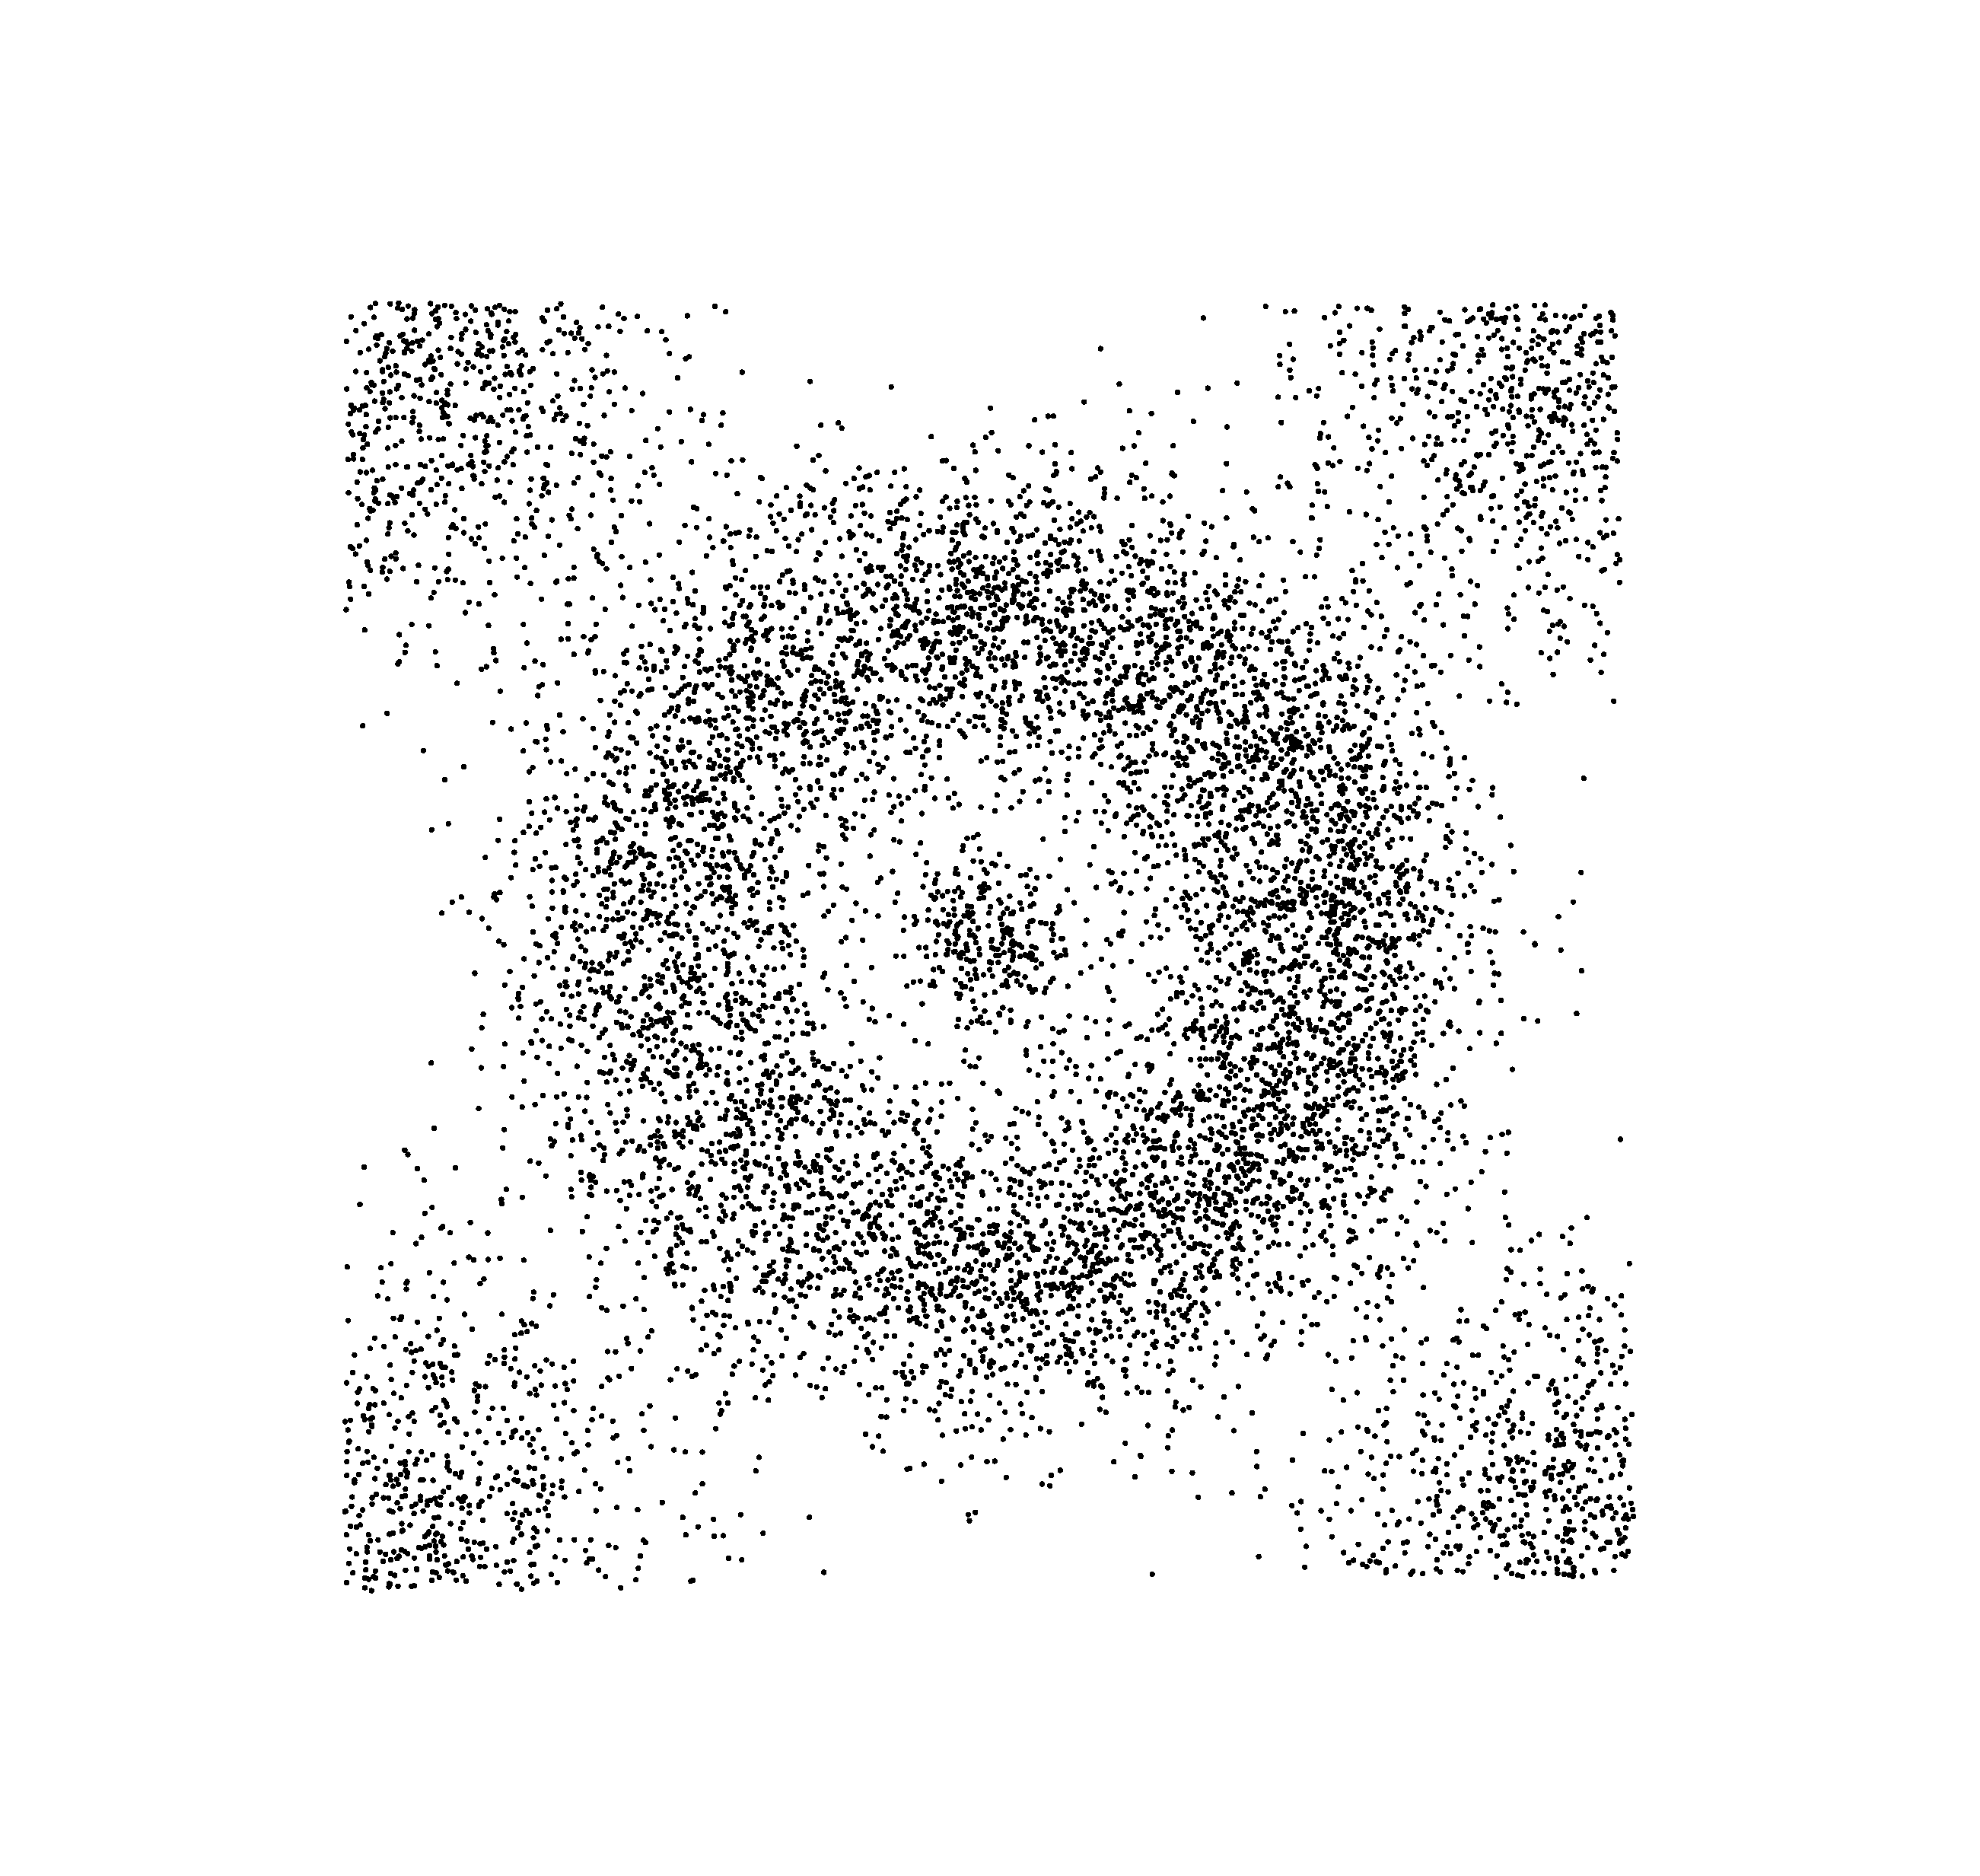
\includegraphics[width=6.5cm]{figures/crater} &\includegraphics[width=3.5cm]{figures/craterDTM_10_40_mappercoord0_subs100_g40.pdf} & \includegraphics[width=5cm]{figures/craterDTM_10_40_conf85_boot100.pdf} \\
\end{tabular}
\caption[Automatic Mappers on a noisy dataset]{\label{fig:noisy} Mappers computed with automatic tuning (middle) and 85 percent confidence regions for their topological features (right) are provided for
a a noisy crater in the Euclidean plane. }
\end{figure}

























\section{Conclusion}


In this chapter, we studied Mappers computed on point clouds. More precisely, we derived approximation results in the deterministic case,
where there is no assumptions on the point cloud generation, and we provided
a statistical analysis of the Mapper when the point cloud is drawn from a probability distribution. 
Namely, we first proved the fact that the Mapper is
a measurable construction %in Proposition~\ref{prop:Measurability}, 
and then we used the approximation results %Theorem~\ref{thm:geomineq} 
to show that the Mapper is a minimax optimal 
estimator of the Reeb graph in various contexts (Propositions~\ref{prop:UpBdRestr},~\ref{prop:lecam} and~\ref{prop:subs})
and that corresponding confidence regions can be computed. %---see Proposition~\ref{prop:conf1} and Section~\ref{sec:bootstrap}.
Along the way, we derived rules of thumb to automatically tune the parameters of the Mapper with Equation~(\ref{ref:coeff_ab_inconnus}), and 
showed their efficiency in a few examples of application of our methods on various datasets. %in Section~\ref{sec:appli}.

Among the future perspectives of this work are the following questions:

\begin{itemize}

\item {\bf Can results from~\cite{Chazal14b} be adapted to  
prove the validity of bootstrap methods?} 
We only used bootstrap methods empirically in this thesis.
As mentioned in Section~\ref{sec:bootstrap}, proving the validity of 
bootstrap in the context for the Mapper 
%for computing confidence regions on the Mapper,
would require to write  
$\dper ( \Map_n^*, \Map_n)$ in terms of the distance between the extrema of the filter function and 
the ones of the interpolation of the filter function on the Rips graph.

\item {\bf Is it possible to weight the Rips graph?}
Using weighted Rips complexes~\cite{Buchet15} instead of the usual Rips complexes might
improve the quality of the confidence regions on the Mapper features,
and would probably be a better way to deal with noise than our current solution.

\item {\bf Is there applications in feature selection?}
It would be interesting to check whether  our statistical setting can be adapted to the question of selecting variables,
which is one of the main applications of the Mapper in practice.

\end{itemize}

%\bibliographystyle{plain}
%\bibliography{biblio}
